%% MADKE-X manuscript -- Elsevier elsarticle template (Neurocomputing).
%% Compile: pdflatex -> bibtex -> pdflatex -> pdflatex (VS Code LaTeX Workshop does this on save;
%% Overleaf does it automatically).
%%
%% NUMBERS, RESULT TABLES AND RESULT FIGURES ARE GENERATED, NOT TYPED:
%%   python run_experiments.py --mode offline     (writes results/offline/tables.json)
%%   python paper_assets.py                       (writes overleaf/generated/*.tex and overleaf/figures/fig_*.pdf)
%% In the text a number looks like \VGainTQA{}; its value is defined in generated/numbers.tex.
\documentclass[preprint,12pt]{elsarticle}

\usepackage[T1]{fontenc}
\usepackage{lmodern}
\usepackage{microtype}
\usepackage{amsmath,amssymb}
\usepackage{graphicx}
\usepackage{booktabs}
\usepackage{multirow}
\usepackage{array}
\usepackage{xcolor}
\usepackage[ruled,vlined,linesnumbered]{algorithm2e}
\usepackage{tikz}
\usetikzlibrary{arrows.meta,positioning,fit,backgrounds,calc,shapes.geometric}
\usepackage[hidelinks]{hyperref}

\graphicspath{{figures/}}
\SetKwInOut{Input}{Input}
\SetKwInOut{Output}{Output}
\newcommand{\flag}[1]{\texttt{-{}-#1}}
\setlength{\emergencystretch}{1.5em}
% let floats share a page with text instead of taking a page of their own
\renewcommand{\topfraction}{0.9}
\renewcommand{\bottomfraction}{0.8}
\renewcommand{\textfraction}{0.08}
\renewcommand{\floatpagefraction}{0.85}
\setcounter{topnumber}{3}
\setcounter{bottomnumber}{2}
\setcounter{totalnumber}{4}
\setlength{\belowcaptionskip}{6pt}

% generated by paper_assets.py -- do not edit by hand
% every number of the running text; write \VName{} when a space follows
\newcommand{\VNPerSet}{500}
\newcommand{\VNQuestions}{2,500}
\newcommand{\VCodeVersion}{1.2.0}
\newcommand{\VPython}{3.12.10}
\newcommand{\VElapsed}{180}
\newcommand{\VSelRel}{11,324}
\newcommand{\VSetOkRel}{10,447}
\newcommand{\VSetBadRel}{877}
\newcommand{\VSetPctRel}{92.3}
\newcommand{\VOrderOkRel}{18}
\newcommand{\VOrderPctRel}{0.2}
\newcommand{\VBindRel}{0}
\newcommand{\VStopOkRel}{1,655}
\newcommand{\VStopPctRel}{66.2}
\newcommand{\VStopLateRel}{845}
\newcommand{\VJudgeRepliesRel}{5,662}
\newcommand{\VJudgeYesRel}{3,181}
\newcommand{\VMissedRel}{1,348}
\newcommand{\VMissedPctRel}{42.4}
\newcommand{\VFalseAgreeRel}{0}
\newcommand{\VDroppedRel}{0}
\newcommand{\VOutRangeRel}{0}
\newcommand{\VNotFoundRel}{0}
\newcommand{\VIgnoredRel}{0}
\newcommand{\VUnparsedRel}{0}
\newcommand{\VConsTrueRel}{89.4}
\newcommand{\VConsPipeRel}{73.3}
\newcommand{\VConsFormRel}{54.6}
\newcommand{\VCoTrueRel}{11.7}
\newcommand{\VCoPipeRel}{9.9}
\newcommand{\VCoFormRel}{8.3}
\newcommand{\VRoundsRel}{2.26}
\newcommand{\VCallsRel}{12.3}
\newcommand{\VInTokRel}{12,420}
\newcommand{\VFailedRel}{0}
\newcommand{\VSelX}{7,992}
\newcommand{\VSetOkX}{7,992}
\newcommand{\VSetBadX}{0}
\newcommand{\VSetPctX}{100.0}
\newcommand{\VOrderOkX}{7,992}
\newcommand{\VOrderPctX}{100.0}
\newcommand{\VBindX}{2,500}
\newcommand{\VStopOkX}{2,500}
\newcommand{\VStopPctX}{100.0}
\newcommand{\VStopLateX}{0}
\newcommand{\VJudgeRepliesX}{3,996}
\newcommand{\VJudgeYesX}{2,397}
\newcommand{\VMissedX}{997}
\newcommand{\VMissedPctX}{41.6}
\newcommand{\VFalseAgreeX}{5}
\newcommand{\VDroppedX}{935}
\newcommand{\VOutRangeX}{785}
\newcommand{\VNotFoundX}{2}
\newcommand{\VIgnoredX}{2}
\newcommand{\VUnparsedX}{0}
\newcommand{\VConsTrueX}{95.9}
\newcommand{\VConsPipeX}{95.9}
\newcommand{\VConsFormX}{94.4}
\newcommand{\VCoTrueX}{12.3}
\newcommand{\VCoPipeX}{12.3}
\newcommand{\VCoFormX}{12.1}
\newcommand{\VRoundsX}{1.60}
\newcommand{\VCallsX}{9.0}
\newcommand{\VInTokX}{6,642}
\newcommand{\VFailedX}{0}
\newcommand{\VInTokRed}{46.5}
\newcommand{\VConsGapMin}{25.0}
\newcommand{\VConsGapMax}{40.0}
\newcommand{\VConsGapXMin}{1.0}
\newcommand{\VConsGapXMax}{2.2}
\newcommand{\VTokRelTQA}{1,671}
\newcommand{\VTokSpecTQA}{926}
\newcommand{\VTokXTQA}{923}
\newcommand{\VTokRedTQA}{44.8}
\newcommand{\VDupTQA}{12}
\newcommand{\VConsTrueRelTQA}{91.6}
\newcommand{\VConsFormRelTQA}{54.8}
\newcommand{\VConsXTQA}{95.2}
\newcommand{\VScriptEmRelTQA}{15.0}
\newcommand{\VScriptEmXTQA}{16.2}
\newcommand{\VScriptPTQA}{\ensuremath{0.55}}
\newcommand{\VTokRelNQ}{1,669}
\newcommand{\VTokSpecNQ}{932}
\newcommand{\VTokXNQ}{930}
\newcommand{\VTokRedNQ}{44.3}
\newcommand{\VDupNQ}{12}
\newcommand{\VConsTrueRelNQ}{90.8}
\newcommand{\VConsFormRelNQ}{50.8}
\newcommand{\VConsXNQ}{94.0}
\newcommand{\VScriptEmRelNQ}{7.2}
\newcommand{\VScriptEmXNQ}{8.0}
\newcommand{\VScriptPNQ}{\ensuremath{0.67}}
\newcommand{\VTokRelHQA}{1,713}
\newcommand{\VTokSpecHQA}{954}
\newcommand{\VTokXHQA}{951}
\newcommand{\VTokRedHQA}{44.5}
\newcommand{\VDupHQA}{13}
\newcommand{\VConsTrueRelHQA}{85.0}
\newcommand{\VConsFormRelHQA}{48.6}
\newcommand{\VConsXHQA}{97.2}
\newcommand{\VScriptEmRelHQA}{3.6}
\newcommand{\VScriptEmXHQA}{3.8}
\newcommand{\VScriptPHQA}{\ensuremath{1.00}}
\newcommand{\VTokRelWMQ}{1,761}
\newcommand{\VTokSpecWMQ}{981}
\newcommand{\VTokXWMQ}{977}
\newcommand{\VTokRedWMQ}{44.5}
\newcommand{\VDupWMQ}{16}
\newcommand{\VConsTrueRelWMQ}{81.8}
\newcommand{\VConsFormRelWMQ}{45.8}
\newcommand{\VConsXWMQ}{95.4}
\newcommand{\VScriptEmRelWMQ}{0.0}
\newcommand{\VScriptEmXWMQ}{0.0}
\newcommand{\VScriptPWMQ}{\ensuremath{1.00}}
\newcommand{\VTokRelFEV}{1,685}
\newcommand{\VTokSpecFEV}{937}
\newcommand{\VTokXFEV}{935}
\newcommand{\VTokRedFEV}{44.5}
\newcommand{\VDupFEV}{7}
\newcommand{\VConsTrueRelFEV}{98.0}
\newcommand{\VConsFormRelFEV}{73.0}
\newcommand{\VConsXFEV}{97.6}
\newcommand{\VScriptEmRelFEV}{33.6}
\newcommand{\VScriptEmXFEV}{34.6}
\newcommand{\VScriptPFEV}{\ensuremath{0.30}}
\newcommand{\VNSpanTQA}{500}
\newcommand{\VNVerdictGoldTQA}{0}
\newcommand{\VCovOneOrigTQA}{39.2}
\newcommand{\VCovOneRrfTQA}{56.4}
\newcommand{\VCovOneBmTQA}{54.8}
\newcommand{\VCovOneInterTQA}{39.2}
\newcommand{\VCovOneRandTQA}{39.3}
\newcommand{\VCovThreeOrigTQA}{52.0}
\newcommand{\VCovThreeRrfTQA}{76.0}
\newcommand{\VCovThreeBmTQA}{75.8}
\newcommand{\VCovThreeInterTQA}{72.6}
\newcommand{\VCovThreeRandTQA}{66.5}
\newcommand{\VCovFiveOrigTQA}{57.0}
\newcommand{\VCovFiveRrfTQA}{79.2}
\newcommand{\VCovFiveBmTQA}{80.2}
\newcommand{\VCovFiveInterTQA}{78.8}
\newcommand{\VCovFiveRandTQA}{76.1}
\newcommand{\VMrrOrigTQA}{0.486}
\newcommand{\VMrrRrfTQA}{0.666}
\newcommand{\VGainTQA}{24.0}
\newcommand{\VGainLoTQA}{19.8}
\newcommand{\VGainHiTQA}{28.4}
\newcommand{\VRrfOnlyTQA}{130}
\newcommand{\VOrigOnlyTQA}{10}
\newcommand{\VPvalTQA}{\ensuremath{8.9\times10^{-28}}}
\newcommand{\VCoverRelTQA}{83.8}
\newcommand{\VCoverXTQA}{83.0}
\newcommand{\VCoverLossTQA}{0.8}
\newcommand{\VStressBeforeTQA}{70.3}
\newcommand{\VStressAfterTQA}{99.6}
\newcommand{\VSupXTQA}{99.6}
\newcommand{\VNSpanNQ}{500}
\newcommand{\VNVerdictGoldNQ}{0}
\newcommand{\VCovOneOrigNQ}{47.2}
\newcommand{\VCovOneRrfNQ}{45.0}
\newcommand{\VCovOneBmNQ}{35.4}
\newcommand{\VCovOneInterNQ}{47.2}
\newcommand{\VCovOneRandNQ}{30.1}
\newcommand{\VCovThreeOrigNQ}{60.4}
\newcommand{\VCovThreeRrfNQ}{66.4}
\newcommand{\VCovThreeBmNQ}{63.2}
\newcommand{\VCovThreeInterNQ}{69.4}
\newcommand{\VCovThreeRandNQ}{57.3}
\newcommand{\VCovFiveOrigNQ}{67.6}
\newcommand{\VCovFiveRrfNQ}{75.4}
\newcommand{\VCovFiveBmNQ}{73.8}
\newcommand{\VCovFiveInterNQ}{76.2}
\newcommand{\VCovFiveRandNQ}{69.7}
\newcommand{\VMrrOrigNQ}{0.565}
\newcommand{\VMrrRrfNQ}{0.578}
\newcommand{\VGainNQ}{6.0}
\newcommand{\VGainLoNQ}{1.6}
\newcommand{\VGainHiNQ}{10.4}
\newcommand{\VRrfOnlyNQ}{75}
\newcommand{\VOrigOnlyNQ}{45}
\newcommand{\VPvalNQ}{\ensuremath{0.008}}
\newcommand{\VCoverRelNQ}{86.6}
\newcommand{\VCoverXNQ}{83.6}
\newcommand{\VCoverLossNQ}{3.0}
\newcommand{\VStressBeforeNQ}{61.8}
\newcommand{\VStressAfterNQ}{99.6}
\newcommand{\VSupXNQ}{99.6}
\newcommand{\VNSpanHQA}{465}
\newcommand{\VNVerdictGoldHQA}{35}
\newcommand{\VCovOneOrigHQA}{16.1}
\newcommand{\VCovOneRrfHQA}{27.5}
\newcommand{\VCovOneBmHQA}{22.6}
\newcommand{\VCovOneInterHQA}{16.1}
\newcommand{\VCovOneRandHQA}{13.4}
\newcommand{\VCovThreeOrigHQA}{21.7}
\newcommand{\VCovThreeRrfHQA}{41.5}
\newcommand{\VCovThreeBmHQA}{39.4}
\newcommand{\VCovThreeInterHQA}{34.6}
\newcommand{\VCovThreeRandHQA}{28.7}
\newcommand{\VCovFiveOrigHQA}{24.9}
\newcommand{\VCovFiveRrfHQA}{45.8}
\newcommand{\VCovFiveBmHQA}{45.2}
\newcommand{\VCovFiveInterHQA}{40.2}
\newcommand{\VCovFiveRandHQA}{37.2}
\newcommand{\VMrrOrigHQA}{0.219}
\newcommand{\VMrrRrfHQA}{0.348}
\newcommand{\VGainHQA}{19.8}
\newcommand{\VGainLoHQA}{16.1}
\newcommand{\VGainHiHQA}{23.9}
\newcommand{\VRrfOnlyHQA}{100}
\newcommand{\VOrigOnlyHQA}{8}
\newcommand{\VPvalHQA}{\ensuremath{2.4\times10^{-21}}}
\newcommand{\VCoverRelHQA}{51.6}
\newcommand{\VCoverXHQA}{48.2}
\newcommand{\VCoverLossHQA}{3.4}
\newcommand{\VStressBeforeHQA}{74.4}
\newcommand{\VStressAfterHQA}{99.6}
\newcommand{\VSupXHQA}{99.6}
\newcommand{\VNSpanWMQ}{468}
\newcommand{\VNVerdictGoldWMQ}{32}
\newcommand{\VCovOneOrigWMQ}{6.4}
\newcommand{\VCovOneRrfWMQ}{16.2}
\newcommand{\VCovOneBmWMQ}{18.8}
\newcommand{\VCovOneInterWMQ}{6.4}
\newcommand{\VCovOneRandWMQ}{7.2}
\newcommand{\VCovThreeOrigWMQ}{11.8}
\newcommand{\VCovThreeRrfWMQ}{26.3}
\newcommand{\VCovThreeBmWMQ}{26.5}
\newcommand{\VCovThreeInterWMQ}{22.0}
\newcommand{\VCovThreeRandWMQ}{17.9}
\newcommand{\VCovFiveOrigWMQ}{15.2}
\newcommand{\VCovFiveRrfWMQ}{32.3}
\newcommand{\VCovFiveBmWMQ}{32.1}
\newcommand{\VCovFiveInterWMQ}{29.1}
\newcommand{\VCovFiveRandWMQ}{25.8}
\newcommand{\VMrrOrigWMQ}{0.119}
\newcommand{\VMrrRrfWMQ}{0.228}
\newcommand{\VGainWMQ}{14.5}
\newcommand{\VGainLoWMQ}{10.5}
\newcommand{\VGainHiWMQ}{18.6}
\newcommand{\VRrfOnlyWMQ}{84}
\newcommand{\VOrigOnlyWMQ}{16}
\newcommand{\VPvalWMQ}{\ensuremath{2.6\times10^{-12}}}
\newcommand{\VCoverRelWMQ}{41.2}
\newcommand{\VCoverXWMQ}{38.0}
\newcommand{\VCoverLossWMQ}{3.2}
\newcommand{\VStressBeforeWMQ}{65.1}
\newcommand{\VStressAfterWMQ}{99.6}
\newcommand{\VSupXWMQ}{99.6}
\newcommand{\VWorstGapRrf}{3.0}
\newcommand{\VWorstGapBm}{11.8}
\newcommand{\VWorstGapInter}{17.2}
\newcommand{\VWorstGapOrig}{24.0}
\newcommand{\VGainMin}{6.0}
\newcommand{\VGainMax}{24.0}
\newcommand{\VPvalMax}{\ensuremath{0.008}}
\newcommand{\VHolmMax}{\ensuremath{0.008}}
\newcommand{\VTokRedMin}{44.3}
\newcommand{\VTokRedMax}{44.8}
\newcommand{\VTokRedMean}{44.5}
\newcommand{\VTokRedSpecMax}{0.5}
\newcommand{\VTokSavedMin}{739}
\newcommand{\VTokSavedMax}{784}
\newcommand{\VTokSavedSixMax}{4,703}
\newcommand{\VCoverLossMin}{0.8}
\newcommand{\VCoverLossMax}{3.4}
\newcommand{\VDupMin}{7}
\newcommand{\VDupMax}{16}
\newcommand{\VDupTotal}{60}
\newcommand{\VBuildXMin}{0.64}
\newcommand{\VBuildXMax}{0.78}
\newcommand{\VBuildRelMax}{0.0011}
\newcommand{\VIndexMsMin}{180}
\newcommand{\VIndexMsMax}{197}
\newcommand{\VIndexNMin}{4,770}
\newcommand{\VIndexNMax}{4,996}
\newcommand{\VMemXMin}{2.2}
\newcommand{\VMemXMax}{2.3}
\newcommand{\VMemRelMax}{0.08}
\newcommand{\VSupXMin}{99.6}
\newcommand{\VSupXMax}{99.6}
\newcommand{\VCiteParsed}{3,270}
\newcommand{\VCiteValid}{3,270}
\newcommand{\VVerCalls}{13}
\newcommand{\VVerAdopt}{5}
\newcommand{\VVerAbst}{8}
\newcommand{\VVerdictAnswers}{2}
\newcommand{\VStressApplicable}{1,998}
\newcommand{\VStressCalls}{641}
\newcommand{\VStressAdopt}{633}
\newcommand{\VStressNew}{5}
\newcommand{\VStressSame}{628}
\newcommand{\VStressAbst}{8}
\newcommand{\VStressRejected}{0}
\newcommand{\VStressTouched}{0}
\newcommand{\VStressBeforeMin}{61.8}
\newcommand{\VStressBeforeMax}{74.4}
\newcommand{\VStressAfterMin}{99.6}
\newcommand{\VStressAfterMax}{99.6}
\newcommand{\VFailRate}{2}
\newcommand{\VFailN}{100}
\newcommand{\VFailNAll}{500}
\newcommand{\VFailScoredRel}{100}
\newcommand{\VFailScoredRelMin}{18}
\newcommand{\VFailScoredRelMax}{24}
\newcommand{\VFailMarkedRel}{0}
\newcommand{\VFailFlaggedX}{68}
\newcommand{\VFailFlaggedXMin}{9}
\newcommand{\VFailFlaggedXMax}{16}
\newcommand{\VFailScoredX}{0}
\newcommand{\VInvChecks}{4,003}
\newcommand{\VInvChecksAll}{20,015}
\newcommand{\VInvPassedAll}{20,015}
\newcommand{\VScriptPMin}{\ensuremath{0.30}}
\newcommand{\VPubCells}{95}
\newcommand{\VPubMultiples}{94}
\newcommand{\VPubOdd}{0.625}
\newcommand{\VPowN}{15}
\newcommand{\VPowOver}{11}
\newcommand{\VPowOverTwoK}{8}
\newcommand{\VPowBelow}{2}
\newcommand{\VPowMinResolved}{7.8}
\newcommand{\VPowHalfMargin}{8.8}
\newcommand{\VPairedNeed}{1,011}
\newcommand{\VPairedNeedHalf}{2,025}
\newif\iflivedone
\livedonefalse

\renewcommand{\bibfont}{\small}

\journal{Neurocomputing}

\begin{document}

\begin{frontmatter}

\title{MADKE-X: Traceable, Evidence-Governed Multi-Agent Debate for Knowledge-Intensive Question Answering}

\author[iu]{Muhammad Ali}
\author[iu]{Muhammad Talha}
\affiliation[iu]{organization={Department of Computer Science, Iqra University, Airport Campus},
            city={Karachi},
            country={Pakistan}}

\begin{abstract}
Multi-agent debate over retrieved evidence is a leading approach to factual question answering with large language models, yet current systems give no assurance about the path from evidence to answer. It is not recorded which passages reached an agent, a failed model call can be scored as an answer, and the order of the evidence is left to the retriever. An inspection of the public code of MADKE, a representative system, documents thirteen such weaknesses. This study introduces MADKE-X, a governed debate framework with four components, each defined by equations: a failure-aware interface layer that reports failed calls and reads replies in any common format, an evidence governor that fuses the retrieval rank with a question-only BM25 rank, a decision trace that links every answer to the passages it cites, and a verification step bounded to one extra call. The debate protocol is left untouched, so every effect is attributable to one component. On five unaltered benchmark files, the governor raises the share of questions with an answer-bearing passage among the first three from \VCovThreeOrigTQA\% to \VCovThreeRrfTQA\% on TriviaQA, \VCovThreeOrigNQ\% to \VCovThreeRrfNQ\% on NQ, \VCovThreeOrigHQA\% to \VCovThreeRrfHQA\% on HotpotQA and \VCovThreeOrigWMQ\% to \VCovThreeRrfWMQ\% on 2WikiMultihopQA (paired exact McNemar test, $p\le\VPvalMax$). Under identical scripted agents MADKE-X passes all \VInvChecksAll{} pipeline checks, ends every debate in the round of agreement, where the release does so for \VStopPctRel\%, and needs \VInTokRed\% fewer input tokens per question. A debate system can thus be made auditable, safe against failed calls and markedly cheaper without any change to the debate; accuracy with live models is compared under a paired protocol.
\end{abstract}


\begin{keyword}
multi-agent debate \sep large language models \sep retrieval-augmented generation \sep
reciprocal rank fusion \sep evidence attribution \sep knowledge-intensive question answering
\end{keyword}

\end{frontmatter}

\section{Introduction}
\label{sec:introduction}

Large language models (LLMs) answer factual questions fluently, but fluency is a poor guide to correctness \cite{brown2020gpt3,ji2023hallucination}. A model may repeat an outdated fact, confuse two entities with similar names, or state something plausible that no source supports, and the reader cannot tell which part of the answer rests on evidence. Two families of methods attack this weakness from different sides. Retrieval-augmented generation places passages retrieved from an external corpus in front of the model, so that the answer can be grounded in text outside the model \cite{lewis2020rag,guu2020realm,izacard2021fid}. Multi-agent debate gives the same question to several instances of a model and lets them read and criticise each other's answers over a few rounds, on the premise that one instance catches the errors of another \cite{du2024debate,liang2024divergent,chan2024chateval}.

MADKE \cite{wang2025madke} joins the two ideas. Each question comes with a shared pool of Wikipedia and Google passages. In every round, each debating agent selects at most three passages from the pool, answers with them in view and reads the answers of the other agents. A judge agent decides after the round whether the agents agree, and a summariser agent writes the final answer once they agree or the round budget is used up. The method appeared in \emph{Neurocomputing} and is reported to outperform single-agent prompting, chain-of-thought prompting \cite{wei2022cot}, self-consistency \cite{wang2023sc}, retrieval-augmented generation and plain debate on TriviaQA, Natural Questions, HotpotQA, 2WikiMultihopQA and FEVER with three backbone models.

Other researchers can use a method of this kind only through its implementation. Before MADKE was extended in this study, its public code \cite{madke2025code} was read line by line and its logic was run again under controlled replies. The code does not execute the method as the paper describes it. The call of the summariser passes the debate transcript and the question in the wrong order, so that in every final prompt the line marked ``Question:'' holds the replies of the agents. The parser for the passages an agent selects accepts only brackets that hold a single number: a selection written as one list, such as \texttt{[2, 0, 7]}, delivers no passage at all, and nothing in the output says so. The judge counts as agreeing only if it writes the exact string \texttt{[Yes]}; with \texttt{[yes]} or \texttt{["Yes"]} the debate goes on. The script that computes the consistency statistics never counts an agreement reached in the final round. A failed model call hands back its error message as if it were a reply, and the message is scored as an answer. The default pool is larger than the paper specifies, it can hold the same passage twice, and it is always listed with Wikipedia first. The output keeps the raw prompts and replies, but no structured record of which passages reached which agent and which of them support the final answer. Correctness, cost and auditability are all affected.

These weaknesses are not peculiar to one code base. They follow from a design in which the path from the evidence to the answer is governed by nothing: no component decides in which order the evidence is shown, none records what an agent received, and none notices a call that failed. This study introduces MADKE-X, a governed debate framework that places this path under explicit control. The debate itself is left untouched: the same agents, the same debate prompts, the same round budget. Every measured difference can therefore be attributed to a component of the framework and not to a new debate design. The framework has four components. A failure-aware interface layer makes every model call report success or failure, binds the summariser prompt by keyword, reads the selection of an agent from the end of its reply in any bracket format, reads the last verdict of the judge in any spelling, and computes the debate statistics from stored verdicts. An evidence governor builds the specified pool of five plus five passages, removes duplicates and orders the rest by reciprocal rank fusion \cite{cormack2009rrf} of the retrieval rank and a BM25 rank \cite{robertson2009bm25} computed from the question alone. A decision trace records the pool, the passages delivered in every round, the verdicts and the passages the summariser cites with $\{E\#\}$ markers, together with a lexical check of whether the answer occurs in a cited passage. A bounded verification step calls the summariser once more when that check fails and adopts the second answer only if it passes.

The evaluation separates what can be shown without a language model from what cannot. The five benchmark files shipped with MADKE are used unaltered and are verified by SHA-256 digests before every run. The order of the evidence, the size of the prompts and the cost of the added steps are properties of the data and the code, and they are measured directly on the \VNQuestions{} questions. Whether a pipeline does what it is specified to do is tested with deterministic scripted agents, which drive the release and MADKE-X through replies of known content so that every difference in behaviour is caused by the code. End-to-end accuracy needs a live model. For that comparison both systems answer the same questions with the same open-weight backbone under a paired protocol; its status is reported in Section~\ref{sec:live}.

The contributions are the following.
\begin{enumerate}
\item \emph{A governed debate framework.} MADKE-X is a framework for knowledge-enhanced debate in which every step between the evidence pool and the final answer is specified by an equation, with its symbols and its effect on the results stated (Section~\ref{sec:method}). A complexity analysis bounds the number of model calls per question (Section~\ref{sec:complexity}).
\item \emph{An evidence governor that needs no training.} The governor fuses the rank of the retriever with a BM25 rank computed from the question alone. It lists answer-bearing passages earlier on all four question-answering datasets, by \VGainMin{} to \VGainMax{} percentage points at the first three positions, and shortens the evidence listing by \VTokRedMean\% (Section~\ref{sec:offline}).
\item \emph{Auditable answers.} A decision trace with passage citations links every answer to the evidence that was delivered and cited, and a verification step bounded to one extra call raises the number of supported answers without changing a supported one (Sections~\ref{sec:m_trace} and~\ref{sec:m_verify}).
\item \emph{An evaluation protocol that does not depend on a model.} Deterministic scripted agents drive two systems through replies of known content, so that every difference in behaviour is caused by the code. Paired tests, bootstrap intervals, multiplicity correction and a power analysis make a claimed difference testable (Section~\ref{sec:design}).
\item \emph{An inspection of a public debate system.} The inspection of the MADKE implementation documents thirteen deviations from the published method or weaknesses of its evaluation, each tied to a statement of the code and, where the code can be exercised offline, reproduced by a test (Section~\ref{sec:baseline}).
\item \emph{A strict separation between demonstrated and pending claims.} Accuracy is reported only from live runs of both systems on identical questions, and no accuracy value is estimated or extrapolated (Section~\ref{sec:live}).
\end{enumerate}

The rest of the paper is organised as follows. Section~\ref{sec:related_work} reviews related work. Section~\ref{sec:baseline} describes MADKE and the findings on its implementation. Section~\ref{sec:method} presents MADKE-X with its equations, and Section~\ref{sec:complexity} analyses its cost. Section~\ref{sec:design} sets out the experimental design. Sections~\ref{sec:offline} and~\ref{sec:live} report the offline results and the live comparison, Section~\ref{sec:discussion} discusses them, Section~\ref{sec:threats} lists the threats to validity and Section~\ref{sec:conclusion} concludes.

\section{Related work}
\label{sec:related_work}

Five lines of research meet in MADKE-X: debate among language-model agents, retrieval-augmented generation, the ordering of retrieved evidence, the attribution of answers to sources, and evaluation practice. They are reviewed in turn, and the last subsection states where MADKE-X stands among them.

\subsection{Multi-agent debate and collaboration}
Du et al.~\cite{du2024debate} showed that several instances of a language model that propose answers, read the answers of the others and revise their own over a few rounds reach higher factual accuracy and better arithmetic reasoning than one instance alone. Liang et al.~\cite{liang2024divergent} traced a weakness of self-reflection to what they call degeneration of thought: once a model has committed to an answer, reflecting on it rarely changes its mind. Their remedy is a debate between an affirmative and a negative side, with a judge who ends it. ChatEval \cite{chan2024chateval} used agents with different personas to evaluate generated text and came closer to human judgements than single-agent evaluators did. A more sober picture comes from Smit et al.~\cite{smit2024mad}, who compared debate protocols under matched budgets. In their experiments the benefit of debate depends strongly on the number of agents, the number of rounds and the level of agreement that is enforced, and a tuned single model with self-consistency \cite{wang2023sc} is often as good.

Refinement methods for a single agent rest on the same idea of a second look. Self-Refine \cite{madaan2023selfrefine} has one model criticise and rewrite its own output, Reflexion \cite{shinn2023reflexion} keeps verbal feedback from earlier attempts in memory, and ReAct \cite{yao2023react} alternates reasoning steps with actions such as search queries. All of these methods pass text from one step to the next, and all of them depend on that text being the right one. When a step receives the wrong text, or a reply is parsed wrongly, the second look is applied to the wrong material. MADKE belongs to this family and adds retrieved evidence to the debate. The findings of Section~\ref{sec:baseline} on its public implementation are failures of exactly these text interfaces.

\subsection{Retrieval-augmented generation}
Retrieval-augmented generation (RAG) conditions a generator on passages retrieved from an external corpus. Lewis et al.~\cite{lewis2020rag} combined a dense passage retriever \cite{karpukhin2020dpr} with a sequence-to-sequence generator and trained both together. REALM \cite{guu2020realm} brought retrieval into the pre-training of the language model, and Fusion-in-Decoder \cite{izacard2021fid} showed that a reader can combine many passages when each one is encoded separately. With instruction-following models, retrieval is mostly used without training: the retrieved passages are placed in the prompt. The survey of Gao et al.~\cite{gao2023ragsurvey} sorts such systems into naive, advanced and modular RAG and names the selection, ordering and compression of passages as the main design choices of the advanced kind. For multi-hop questions, IRCoT \cite{trivedi2023ircot} alternates retrieval with chain-of-thought steps, and Self-RAG \cite{asai2024selfrag} trains a model to decide when to retrieve and to judge whether a retrieved passage supports its output.

MADKE uses retrieval in the prompt-based way. Passages were retrieved once per question from Wikipedia and from Google search and are shipped with the benchmark files, and the agents decide which of them to read. What the agents can learn therefore depends on what the pool contains and, as the next subsection argues, on the order in which the pool is listed.

\subsection{Ordering of retrieved evidence}
Liu et al.~\cite{liu2024lost} found that language models use long contexts unevenly: accuracy is highest when the relevant passage stands at the beginning or the end of the context and falls when it stands in the middle. In MADKE an agent sees the whole pool when it selects passages, so the position of an answer-bearing passage in the listing may decide whether the passage is selected. Two classical tools order candidates without labels. BM25 \cite{robertson2009bm25} scores a passage by the frequency of the query terms in it, weighted by their rarity in the collection and normalised by the length of the passage. Reciprocal rank fusion (RRF) \cite{cormack2009rrf} combines several rankings by summing, for each item, the reciprocal of a constant plus its rank in each list. RRF needs no training data, and Cormack et al.\ found it better than the individual rankings and than learned fusion methods. MADKE-X fuses the retrieval rank shipped with the data with a BM25 rank computed from the question, so the order of the pool uses neither a gold answer nor a model.

\subsection{Attribution, hallucination and verification}
A generated answer can be wrong although the correct evidence is in the context \cite{ji2023hallucination}. ALCE \cite{gao2023alce} is a benchmark in which a model must cite the passages that support each of its statements, scored by citation recall and precision. Rashkin et al.~\cite{rashkin2023attribution} define attribution to identified sources as a property that humans can judge and models can approximate. FActScore \cite{min2023factscore} splits a long answer into atomic facts and checks each against a knowledge source, and SelfCheckGPT \cite{manakul2023selfcheckgpt} detects unsupported statements by sampling several answers and measuring their agreement, without external evidence. Jacovi and Goldberg \cite{jacovi2020faithful} add a conceptual point: an explanation is faithful only if it reflects the process that produced the decision.

MADKE-X takes a narrow position here. Its decision trace records what the pipeline did, which makes the trace faithful to the process by construction, and its support check is a lexical test of whether the answer string occurs in a cited passage. The test is cheap and deterministic. It detects a missing answer string and nothing more; in particular it does not establish entailment. A learned attribution model could take its place without any other change to the method.

\subsection{Reproducible and statistically sound evaluation}
Pineau et al.~\cite{pineau2021reproducibility} describe a reproducibility checklist for machine-learning research that asks, among other items, for released code, exact data versions and the number of evaluation runs. Dror et al.~\cite{dror2018hitchhiker} review significance testing in natural language processing and recommend paired tests whenever two systems answer the same items. For binary outcomes on the same questions, the exact McNemar test \cite{mcnemar1947} compares the discordant pairs. The bootstrap \cite{efron1979bootstrap} gives confidence intervals without distributional assumptions, power analysis \cite{cohen1988power} gives the sample size needed to detect a given difference, and the Holm procedure \cite{holm1979} controls the family-wise error rate when several datasets are tested. Exact match (EM) and token-level F1 for extractive question answering follow the SQuAD definitions \cite{rajpurkar2016squad}. A language model used as a judge of correctness shows position and verbosity biases, so its agreement with human judgement has to be checked before its scores are trusted \cite{zheng2023judge}. The protocol of this study follows these recommendations and scores answers with EM and F1, which need no model as judge.

\subsection{Position of MADKE-X}
Table~\ref{tab:positioning} compares representative methods by what they provide. Debate methods without retrieval rely on what the model already knows. Retrieval methods with one model have no second agent that could object. ALCE adds citations but no debate. Among the methods in the table only MADKE combines debate with evidence selection by each agent. MADKE-X adds citations at the level of the answer, a bounded verification step and explicit handling of failed calls, and it leaves the debate as it is.

\begin{table}[!htbp]
\centering
\small
\caption{Capabilities of representative methods (\checkmark{} = provided by the method as published).}
\label{tab:positioning}
\setlength{\tabcolsep}{4pt}
\resizebox{\textwidth}{!}{%
\begin{tabular}{lcccccc}
\toprule
Method & \shortstack{Multiple\\agents} & \shortstack{External\\evidence} & \shortstack{Per-agent\\selection} & \shortstack{Answer\\citations} & \shortstack{Bounded\\verification} & \shortstack{Failure\\handling} \\
\midrule
Multi-agent debate \cite{du2024debate} & \checkmark & & & & & \\
Debate with judge \cite{liang2024divergent} & \checkmark & & & & & \\
RAG \cite{lewis2020rag} & & \checkmark & & & & \\
ALCE \cite{gao2023alce} & & \checkmark & & \checkmark & & \\
MADKE \cite{wang2025madke} & \checkmark & \checkmark & \checkmark & & & \\
MADKE-X (this study) & \checkmark & \checkmark & \checkmark & \checkmark & \checkmark & \checkmark \\
\bottomrule
\end{tabular}%
}
\end{table}

\section{The MADKE baseline}
\label{sec:baseline}

This section describes MADKE as published \cite{wang2025madke}, the data shipped with it, and what an inspection of its public implementation found. The method is described from the paper and the implementation from the released repository \cite{madke2025code} at commit \texttt{9cd57ca}. The data files of that repository are used unaltered throughout this study.

\subsection{Debate procedure}
Let $q$ be a question and $E$ a pool of retrieved passages. MADKE runs $A$ debating agents for at most $R$ rounds. In every round, each agent $i \in \{1,\dots,A\}$ makes two model calls. In the first, the agent sees the whole pool, each passage preceded by its index in square brackets, together with its own previous answer. It is asked to think step by step and to return the indices of up to three helpful passages in square brackets, or to add the marker \texttt{[No Found]} at the end of its reply when the pool holds nothing useful. In the second call, the agent sees the passages it selected, its own previous answer and the answers of the other agents, and writes a new answer that ends with the final answer in square brackets. When all agents have answered, a judge agent receives the question and the answers and replies with \texttt{[Yes]} if the answers agree and with \texttt{[No]} otherwise. When the judge replies \texttt{[Yes]}, or when the last round is reached, a summariser agent receives the question and the debate transcript and writes the final answer, again in square brackets.

With $A$ agents and $R$ rounds, the number of model calls per question is at most
\begin{equation}
C_{\max} = R\,(2A + 1) + 1,
\label{eq:calls}
\end{equation}
where $2A$ counts the selection and answer calls of the agents in one round, the term $1$ inside the parentheses counts the judge, and the final $1$ counts the summariser. The published setting is $A{=}2$, $R{=}3$ and temperature 0.5, which gives $C_{\max} = 16$. A debate that the judge ends before round $R$ uses fewer calls.

\subsection{Benchmarks and evidence pools}
MADKE is evaluated on TriviaQA \cite{joshi2017triviaqa}, Natural Questions (NQ) \cite{kwiatkowski2019nq}, HotpotQA \cite{yang2018hotpotqa}, 2WikiMultihopQA \cite{ho2020twowiki}, FEVER \cite{thorne2018fever} and a medical multiple-choice set, with 500 sampled questions per dataset and 595 for the medical set. The repository ships the first five as JSON files of 500 records each. A record holds the question, the gold answers, ten Wikipedia passages found by dense passage retrieval \cite{karpukhin2020dpr} and up to ten Google search snippets, each list in retrieval order. A Wikipedia passage has about 100 words and a Google snippet about 25. The medical set is not shipped and lies outside this study.

FEVER differs from the other four datasets. Its gold labels are the verdicts \texttt{SUPPORTS}, \texttt{REFUTES} and \texttt{NOT ENOUGH INFO} (168, 166 and 166 claims) and not answer strings, so it is scored by exact match on the label, and measures that look for an answer string in a passage do not apply to it. The same holds for the \VNVerdictGoldHQA{} HotpotQA and \VNVerdictGoldWMQ{} 2WikiMultihopQA questions whose gold answer is ``yes'' or ``no''. They are left out of those measures, which then cover \VNSpanHQA{} and \VNSpanWMQ{} questions of the two datasets.

The paper specifies a pool of the top five Wikipedia passages and five Google results per question. The shipped files bound what any method can reach on them. Even in the larger pool of ten Wikipedia and five Google passages, a passage that contains a gold answer exists for \VCoverRelTQA\% of the TriviaQA and \VCoverRelNQ\% of the NQ questions, but only for \VCoverRelHQA\% of the HotpotQA and \VCoverRelWMQ\% of the 2WikiMultihopQA questions (Table~\ref{tab:pool} in Section~\ref{sec:offline}). On the two multi-hop datasets no ordering or selection method can lift this ceiling.

\subsection{Evaluation as published}
The paper reports token-level F1 and a GPT-4 correctness score for the four question-answering datasets and exact match for FEVER. The backbones are GPT-3.5-Turbo, Qwen1.5-32B-Chat and Qwen1.5-72B-Chat, with GPT-4-Turbo as a single-agent reference. Two statistics describe the debate. The consistency ratio (Cons) is the share of questions on which the agents reached agreement, and the consistent-and-correct ratio (Co2) is the share on which they agreed on a correct answer. The difference between the two is the share of questions on which the agents agreed on a wrong answer. All results are point estimates; the paper gives no confidence intervals and no significance tests.

\subsection{Inspection of the public implementation}
\label{sec:audit}
The repository was read at the commit named above, and each finding below refers to a statement of its code. The findings on the parsers, the summariser call, the consistency statistics and the handling of errors were also reproduced, by unit tests of the affected functions and by running the logic of the release again under scripted agents (Section~\ref{sec:design}). Table~\ref{tab:defects} lists the findings with their consequence and with the part of MADKE-X that addresses them. Findings C1--C8 concern the code of the debate and of its evaluation, P1--P3 the evidence pool, R1 the reporting and X1 the output.

\begin{table}[!htbp]
\centering
\footnotesize
\caption{Findings on the public MADKE release (commit \texttt{9cd57ca}) and the part of MADKE-X that addresses each.}
\label{tab:defects}
\setlength{\tabcolsep}{4pt}
\begin{tabular}{p{0.035\textwidth}>{\raggedright\arraybackslash}p{0.37\textwidth}>{\raggedright\arraybackslash}p{0.33\textwidth}>{\raggedright\arraybackslash}p{0.17\textwidth}}
\toprule
ID & Finding & Consequence & Addressed by \\
\midrule
C1 & The summariser is called with the debate transcript and the question in swapped positions. & The line ``Question:'' of every summariser prompt holds the replies of the agents. & Keyword binding (Sec.~\ref{sec:m_interface}) \\
C2 & The test file is read with the slice \texttt{[59:]}. & An unmodified run answers 441 of the 500 questions. & Explicit index range \\
C3 & The selection parser reads only brackets that hold one integer and one spelling of the not-found marker; passages are delivered in reverse order. & A list in one bracket delivers no passage; a marker in another spelling is ignored. & Eq.~\eqref{eq:parse} \\
C4 & The judge counts as agreeing only if a bracket holds exactly \texttt{Yes}. & \texttt{[yes]}, \texttt{["Yes"]} and \texttt{[Yes.]} count as disagreement; a repeated agent answer \texttt{[Yes]} counts as agreement. & Eq.~\eqref{eq:verdict} \\
C5 & The evaluation script looks for \texttt{[Yes]} among the keys of the dictionary that stores the last round. & Agreement reached in the last round is never counted in Cons. & Eq.~\eqref{eq:cons} \\
C6 & Co2 uses the same flag and a GPT-4 judgement of correctness. & Co2 inherits C5 and needs a paid model. & Eq.~\eqref{eq:cons} with exact match \\
C7 & A failed request is retried by unbounded recursion; TLS certificates are not verified. & A persistent failure blocks the run; the server is not authenticated. & Eq.~\eqref{eq:call} \\
C8 & An error object of the API becomes the reply (its message, or the word \texttt{Error}). & Error text enters the debate and is scored as an answer. & Eqs.~\eqref{eq:call}--\eqref{eq:status} \\
\midrule
P1 & The default pool has 10 Wikipedia and 5 Google passages; the paper specifies 5 and 5. & MADKE-X lists \VTokRedMean\% fewer tokens per selection call (Table~\ref{tab:pool}). & Eq.~\eqref{eq:pool} \\
P2 & Duplicate passages are not removed. & \VDupTotal{} passages of the specified pools repeat an earlier passage. & Eq.~\eqref{eq:dedup} \\
P3 & Wikipedia passages are listed first for every question. & Answer-bearing passages, often Google snippets, come late (Table~\ref{tab:ordering}). & Eqs.~\eqref{eq:bm25}--\eqref{eq:rrf} \\
\midrule
R1 & Results are point estimates without intervals or tests. & \VPowOver{} of \VPowN{} published margins need more than 500 questions (Figure~\ref{fig:power}). & Paired protocol (Sec.~\ref{sec:design}) \\
X1 & The output holds the raw prompts and replies only. & No structured link leads from an answer to its evidence. & Trace, Eq.~\eqref{eq:support} \\
\bottomrule
\end{tabular}
\end{table}

Three remarks put the table in perspective. First, the findings describe the code that is published. They do not show which code produced the published numbers, and finding C2 is a case in point. The shares printed in the main table of the paper are multiples of $1/500$ in \VPubMultiples{} of \VPubCells{} cells (the exception is \VPubOdd). This fits an evaluation on 500 questions; shares of 441 questions would end in an odd digit about half of the time. The slice is therefore most probably a leftover of an interrupted run that was resumed. It matters for those who run the release today, not for the published table.

Second, some choices of the release are sensible and are kept. Reading the selection from the end of the reply suits an agent that reasons first and concludes last. MADKE-X keeps this reading and only widens what counts as a selection (Section~\ref{sec:m_interface}).

Third, the findings interact. With C3, an agent that writes its selection as a list reads no evidence in that round. With C4 and C5, debates run longer than needed and the reported consistency is too low. With C1, the final answer is written from a mislabelled prompt even when the debate went well, and with C8 a temporary failure of the API becomes a wrong answer instead of a missing one. None of these effects depends on the quality of the backbone model, which is why they can be measured offline with scripted agents (Section~\ref{sec:offline}).

\section{The proposed method: MADKE-X}
\label{sec:method}

MADKE-X leaves the debate of MADKE as it is and changes what surrounds it. The agents, the debate prompts, the round budget and the order of selecting, answering, judging and summarising are those of Section~\ref{sec:baseline}. Four components are added, and each one answers a group of the findings in Table~\ref{tab:defects}. The \emph{failure-aware interface layer} (Section~\ref{sec:m_interface}) governs the text that passes between the model and the pipeline: every call reports success or failure, the selection of an agent and the verdict of the judge are read in any common format, and the debate statistics are computed from stored verdicts. The \emph{evidence governor} (Section~\ref{sec:m_governor}) decides which passages enter the pool and in which order they are listed. The \emph{decision trace with citations} (Section~\ref{sec:m_trace}) records what the pipeline did for a question and checks whether the final answer occurs in the passages the summariser cites. The \emph{bounded verification step} (Section~\ref{sec:m_verify}) gives the summariser one more attempt when that check fails. Figure~\ref{fig:architecture} shows the complete method, from the shipped question and passage lists to the final answer and its trace, and Table~\ref{tab:notation} lists the symbols. Every equation below corresponds to one function of the released code. After the symbols of an equation are defined, a paragraph headed \emph{Effect on the results} states what the equation changes; the measurements behind these statements are reported in Section~\ref{sec:offline}.

\begin{figure}[!htbp]
\centering
\resizebox{\textwidth}{!}{%
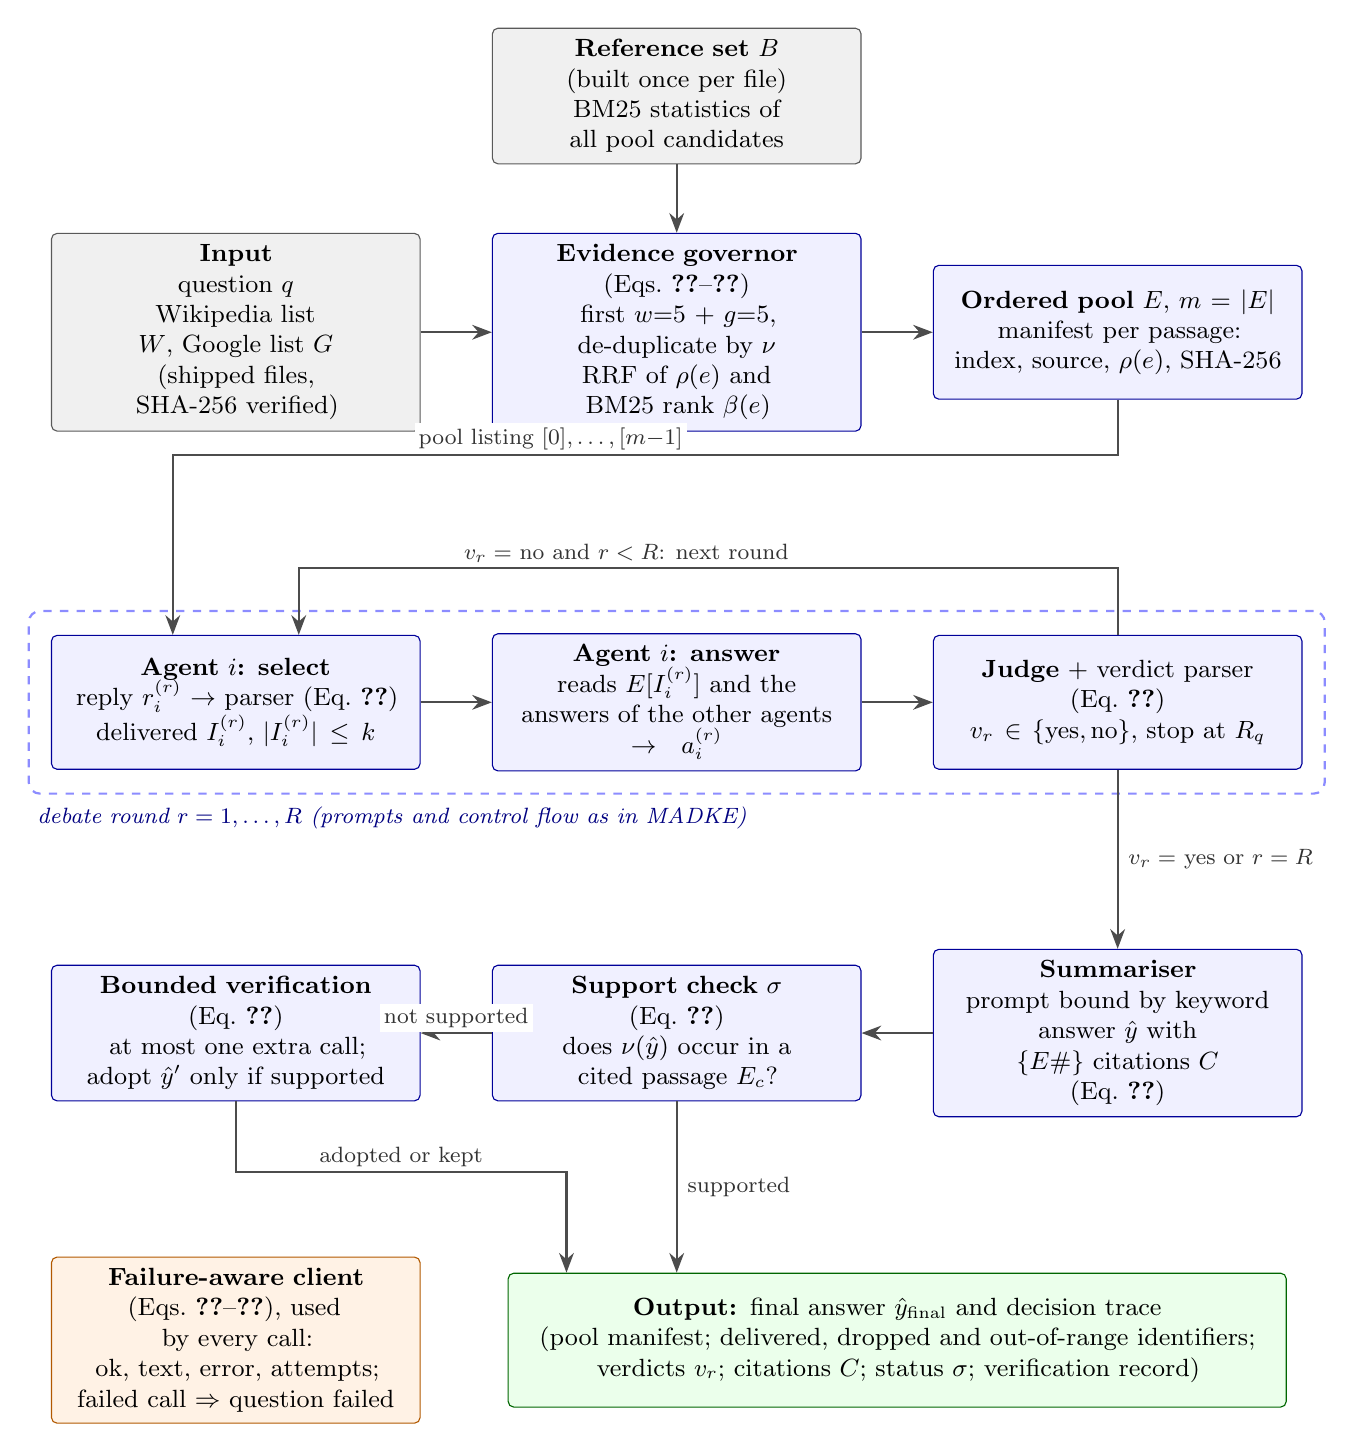
\begin{tikzpicture}[font=\small,
  box/.style={draw=blue!60!black, fill=blue!6, rounded corners=2pt, align=center, minimum height=1.7cm, text width=4.4cm, inner sep=4pt},
  inbox/.style={box, draw=gray!70!black, fill=gray!12},
  outbox/.style={box, draw=green!40!black, fill=green!8},
  clibox/.style={box, draw=orange!70!black, fill=orange!10},
  arr/.style={-{Stealth[length=2.5mm]}, thick, black!70},
  lbl/.style={font=\footnotesize, text=black!80, fill=white, inner sep=1.5pt}]
% row 0: reference statistics
\node[inbox, minimum height=1.2cm] (ref) at (5.6,3.0) {\textbf{Reference set} $B$ (built once per file)\\ BM25 statistics of all pool candidates};
% row 1: input and evidence governor
\node[inbox] (in) at (0,0) {\textbf{Input}\\ question $q$\\ Wikipedia list $W$, Google list $G$\\ (shipped files, SHA-256 verified)};
\node[box] (gov) at (5.6,0) {\textbf{Evidence governor}\\ (Eqs.~\ref{eq:pool}--\ref{eq:rrf})\\ first $w{=}5$ + $g{=}5$, de-duplicate by $\nu$\\ RRF of $\rho(e)$ and BM25 rank $\beta(e)$};
\node[box] (pool) at (11.2,0) {\textbf{Ordered pool} $E$, $m=|E|$\\ manifest per passage:\\ index, source, $\rho(e)$, SHA-256};
% row 2: debate round
\node[box] (sel) at (0,-4.7) {\textbf{Agent $i$: select}\\ reply $r_i^{(r)}$ $\rightarrow$ parser (Eq.~\ref{eq:parse})\\ delivered $I_i^{(r)}$, $|I_i^{(r)}|\le k$};
\node[box] (ans) at (5.6,-4.7) {\textbf{Agent $i$: answer}\\ reads $E[I_i^{(r)}]$ and the\\ answers of the other agents\\ $\rightarrow a_i^{(r)}$};
\node[box] (judge) at (11.2,-4.7) {\textbf{Judge} + verdict parser\\ (Eq.~\ref{eq:verdict})\\ $v_r \in \{\text{yes},\text{no}\}$, stop at $R_q$};
% row 3: summarise, check, verify
\node[box] (summ) at (11.2,-8.9) {\textbf{Summariser}\\ prompt bound by keyword\\ answer $\hat y$ with $\{E\#\}$ citations $C$\\ (Eq.~\ref{eq:cite})};
\node[box] (sup) at (5.6,-8.9) {\textbf{Support check} $\sigma$\\ (Eq.~\ref{eq:support})\\ does $\nu(\hat y)$ occur in a\\ cited passage $E_c$?};
\node[box] (ver) at (0,-8.9) {\textbf{Bounded verification}\\ (Eq.~\ref{eq:verify})\\ at most one extra call;\\ adopt $\hat y'$ only if supported};
% row 4: output and client
\node[outbox, text width=9.6cm] (outn) at (8.4,-12.8) {\textbf{Output:} final answer $\hat y_{\mathrm{final}}$ and decision trace\\ (pool manifest; delivered, dropped and out-of-range identifiers;\\ verdicts $v_r$; citations $C$; status $\sigma$; verification record)};
\node[clibox] (cli) at (0,-12.8) {\textbf{Failure-aware client}\\ (Eqs.~\ref{eq:call}--\ref{eq:emf1}), used by every call:\\ ok, text, error, attempts;\\ failed call $\Rightarrow$ question failed};
% debate frame
\begin{scope}[on background layer]
\node[draw=blue!45, dashed, thick, rounded corners, fit=(sel)(ans)(judge), inner sep=8pt] (deb) {};
\end{scope}
\node[font=\footnotesize\itshape, text=blue!50!black, anchor=north west] at ([yshift=-1pt]deb.south west) {debate round $r = 1,\dots,R$ (prompts and control flow as in MADKE)};
% arrows
\draw[arr] (ref) -- (gov);
\draw[arr] (in) -- (gov);
\draw[arr] (gov) -- (pool);
\draw[arr] (pool.south) -- ++(0,-0.7) -| node[lbl, pos=0.3, above] {pool listing $[0],\dots,[m{-}1]$} ([xshift=-8mm]sel.north);
\draw[arr] (sel) -- (ans);
\draw[arr] (ans) -- (judge);
\draw[arr] (judge.north) -- ++(0,0.85) -| node[lbl, pos=0.3, above] {$v_r=$ no and $r<R$: next round} ([xshift=8mm]sel.north);
\draw[arr] (judge.south) -- node[lbl, right=2pt] {$v_r=$ yes or $r=R$} (summ.north);
\draw[arr] (summ) -- (sup);
\draw[arr] (sup) -- node[lbl, above] {not supported} (ver);
\draw[arr] (sup.south) -- node[lbl, right=2pt] {supported} (sup.south |- outn.north);
\draw[arr] (ver.south) -- ++(0,-0.9) -| node[lbl, pos=0.25, above] {adopted or kept} ([xshift=-4.2cm]outn.north);
\end{tikzpicture}%
}
\caption{Complete methodology of MADKE-X, from the shipped question and passage lists to the final answer and its decision trace. Grey: input as shipped with MADKE and the reference statistics derived from it. Blue: components of the pipeline. Dashed frame: one debate round, with prompts and control flow as in MADKE. Orange: the failure-aware client through which every model call passes. Green: output. Equation numbers refer to Section~\ref{sec:method}.}
\label{fig:architecture}
\end{figure}

\begin{table}[!htbp]
\centering
\small
\caption{Notation.}
\label{tab:notation}
\begin{tabular}{p{0.24\textwidth}p{0.68\textwidth}}
\toprule
Symbol & Meaning \\
\midrule
$q$, $G_q$ & question (or claim, for FEVER) and its set of gold answers \\
$Q$, $Q_c$ & questions evaluated; those whose status is \emph{completed} \\
$A$, $R$, $R_q$ & number of agents (2); maximum number of rounds (3); rounds executed for $q$ \\
$W$, $G$ & Wikipedia and Google passage lists of $q$, in retrieval order \\
$w$, $g$ & number of Wikipedia and Google passages taken (5 and 5) \\
$E=(E_0,\dots,E_{m-1})$ & ordered evidence pool of size $m$ \\
$B$, $N_B$ & reference set of passages for the BM25 statistics; its size \\
$\rho(e)$, $\pi(e)$, $\beta(e)$ & rank of $e$ in its source list; position in the concatenated list; BM25 rank \\
$\nu(\cdot)$ & text normalisation: lower case, punctuation replaced by spaces, whitespace collapsed \\
$k$ & maximum number of passages delivered per selection (3) \\
$r_i^{(r)}$, $I_i^{(r)}$ & selection reply of agent $i$ in round $r$; identifiers delivered to it \\
$U_q$ & union of all $I_i^{(r)}$ for question $q$ \\
$v_r$ & parsed verdict of the judge in round $r$ \\
$\hat y$, $C$, $C^\star$ & answer of the summariser; identifiers it cites; cited identifiers that are valid \\
$\sigma$ & support status of an answer \\
$\mathbb{1}[\cdot]$ & indicator function, 1 if the condition holds and 0 otherwise \\
\bottomrule
\end{tabular}
\end{table}

%% ------------------------------------------------------------------
\subsection{Failure-aware interface layer}
\label{sec:m_interface}

The interface layer sits between the debate and the model server. It has five parts: an explicit result for every model call, keyword binding of the summariser prompt, a parser for the evidence selection, a parser for the verdict of the judge, and the debate statistics computed from the stored verdicts.

\paragraph{Explicit call results and scoring on the completed set}
A call to the model returns a tuple instead of a bare string,
\begin{equation}
\mathrm{call}(\mathbf{m}) = (\mathrm{ok},\; s,\; \epsilon,\; \tau), \qquad 1 \le \tau \le T_{\max}+1,
\label{eq:call}
\end{equation}
where $\mathbf{m}$ is the list of messages sent to the model, $\mathrm{ok}\in\{0,1\}$ states whether a usable reply was received, $s$ is the text of the reply (empty when $\mathrm{ok}=0$), $\epsilon$ describes the error, $\tau$ is the number of attempts made and $T_{\max}$ is the retry budget (three, with exponential back-off). Network errors, time-outs, rate limits, server errors and unreadable responses are retried; other client errors fail at once. The status of a question follows from its mandatory calls, which are the selection, answer, judge and summariser calls:
\begin{equation}
\begin{aligned}
\mathrm{status}(q) &=
\begin{cases}
\text{failed} & \text{if a mandatory call of } q \text{ ends with } \mathrm{ok}=0,\\
\text{completed} & \text{otherwise},
\end{cases}\\
Q_c &= \{q \in Q : \mathrm{status}(q)=\text{completed}\}.
\end{aligned}
\label{eq:status}
\end{equation}
Accuracy is computed on the completed set only. With $\hat y_q$ the final answer of $q$ and $\mathrm{norm}(\cdot)$ the SQuAD answer normalisation \cite{rajpurkar2016squad},
\begin{equation}
\begin{aligned}
\mathrm{EM} &= \frac{1}{|Q_c|}\sum_{q\in Q_c} \max_{g\in G_q} \mathbb{1}\big[\mathrm{norm}(\hat y_q)=\mathrm{norm}(g)\big],\\
\mathrm{F1} &= \frac{1}{|Q_c|}\sum_{q\in Q_c} \max_{g\in G_q} F_1\big(\mathrm{norm}(\hat y_q),\mathrm{norm}(g)\big),
\end{aligned}
\label{eq:emf1}
\end{equation}
where $F_1$ is the harmonic mean of token precision and recall between the prediction and a gold answer. The number of failed questions $|Q\setminus Q_c|$ is reported next to every accuracy value, so a run that loses many questions cannot pass as a clean one.

\emph{Effect on the results.} In the release, a request that raises an exception is repeated without limit, and an error object returned by the server becomes the reply of the agent. The error text then enters the debate, can be taken over by the other agent and is finally scored as a wrong answer (findings C7 and C8). Equations~\eqref{eq:call}--\eqref{eq:emf1} turn such a failure into a counted and excluded question. In the fault-injection experiment of Section~\ref{sec:r_failure}, in which \VFailRate\% of the calls fail, the release scored \VFailScoredRel{} of \VFailNAll{} questions although at least one of their calls had failed and marked none of them. MADKE-X marked \VFailFlaggedX{} questions as failed and scored none of these. Without failures every question completes and Eq.~\eqref{eq:emf1} reduces to the usual definitions. The same client verifies TLS certificates unless the user switches verification off for a local server.

\paragraph{Keyword binding of the summariser prompt}
The summariser prompt has a slot for the question and a slot for the debate transcript. MADKE-X passes both by name, and a positional call is rejected by the interpreter. Each record stores whether the last line of the prompt that starts with ``Question:'' holds the question.

\emph{Effect on the results.} The release passes the two arguments by position and in the wrong order (finding C1). Under scripted agents the question slot holds the question in \VBindRel{} of \VNQuestions{} prompts of the release and in all \VBindX{} prompts of MADKE-X. A swapped prompt still contains the question and the debate, so a capable model may cope with it. How much the swap costs in accuracy is an empirical question for the live comparison.

\paragraph{Evidence selection parser}
Let $\mathrm{br}(r)=(u_1,\dots,u_\ell)$ be the bracket groups of a selection reply $r$ and $Z(r)=(z_1,\dots,z_n)$ the integers that occur in these groups, both in written order. With pool size $m$ and cap $k=3$,
\begin{equation}
\begin{aligned}
\mathrm{NF}(r) &= \mathbb{1}\big[\exists j: u_j \text{ matches } \texttt{no[- ]?found} \text{ (any case)}\big],\\
Z^{\mathrm{in}} &= (z_j : 0\le z_j<m), \qquad D = \mathrm{last}\big(Z^{\mathrm{in}}\big),\\
O &= \mathrm{first}\big((z_j : z_j<0 \,\vee\, z_j\ge m)\big),\\
\mathrm{parse}(r,m,k) &=
\begin{cases}
\big(\varnothing,\ 1,\ D,\ \varnothing,\ O\big) & \text{if } \mathrm{NF}(r)=1,\\
\big(D_{n_D-k+1:n_D},\ 0,\ \varnothing,\ D_{1:n_D-k},\ O\big) & \text{otherwise},
\end{cases}
\end{aligned}
\label{eq:parse}
\end{equation}
where $Z^{\mathrm{in}}$ holds the valid identifiers in written order with repetitions, $\mathrm{last}(\cdot)$ keeps every identifier once, at the position of its last occurrence, $\mathrm{first}(\cdot)$ keeps it at its first occurrence, and $n_D=|D|$. The five components of the result are the delivered identifiers, the not-found flag, the ignored identifiers, the dropped identifiers and the out-of-range identifiers. $D_{n_D-k+1:n_D}$ denotes the last $k$ elements of $D$ (all of $D$ when $n_D\le k$) and $D_{1:n_D-k}$ the elements before them. The identifiers delivered to agent $i$ in round $r$ are $I_i^{(r)} = D_{n_D-k+1:n_D}$, and $U_q=\bigcup_{i,r} I_i^{(r)}$ is their union over all agents and rounds. Algorithm~\ref{alg:parse} gives the procedure.

The parser treats the end of the reply as the selection. The selection prompt asks the agent to think step by step and to put the not-found marker at the end, so an agent may mention passages while it reasons and state its choice last. The same convention holds elsewhere in the pipeline, where the last bracket group is the answer and the last verdict word is the verdict. The release reads the reply from the end as well, and Eq.~\eqref{eq:parse} keeps this choice: for every reply that the release can read, both parsers deliver the same passages. They differ in three respects. Eq.~\eqref{eq:parse} reads the integers inside any bracket group, so a list in one bracket is understood. It recognises the not-found marker in any spelling. And it delivers the passages in the order in which the agent wrote them, where the release delivers them in reverse.

\emph{Effect on the results.} Table~\ref{tab:formats}a shows both parsers on fixed replies. For \texttt{[2, 0, 7]} the release delivers nothing, and the debater then answers without evidence. Under scripted replies whose intended selection is known, the release loses \VSetBadRel{} of \VSelRel{} selections in this way, and MADKE-X loses none of \VSelX{} (Section~\ref{sec:r_interface}). MADKE-X also records what it does not deliver: \VDroppedX{} replies with identifiers beyond the cap and \VOutRangeX{} with identifiers outside the pool. The order of delivery has less weight than the set, since it only changes the sequence in which a debater reads its passages.

\begin{algorithm}[!htbp]
\caption{ParseEvidenceIDs (Eq.~\ref{eq:parse})}
\label{alg:parse}
\Input{reply $r$, pool size $m$, cap $k{=}3$}
\Output{delivered identifiers, not-found flag, ignored, dropped and out-of-range identifiers}
$Z^{\mathrm{in}} \leftarrow [\,]$, $O \leftarrow [\,]$, $f \leftarrow \textbf{false}$\;
\ForEach{bracket group $u$ of $r$, in written order}{
  \lIf{$u$ matches no[- ]?found (any case)}{$f \leftarrow \textbf{true}$}
  \Else{
    \ForEach{integer $z$ in $u$, in written order}{
      \lIf{$0 \le z < m$}{append $z$ to $Z^{\mathrm{in}}$}
      \lElseIf{$z \notin O$}{append $z$ to $O$}
    }
  }
}
$D \leftarrow$ the distinct elements of $Z^{\mathrm{in}}$, each at the position of its last occurrence\;
\lIf{$f$}{\textbf{return} $([\,],\ \textbf{true},\ \text{ignored}=D,\ [\,],\ O)$}
\textbf{return} (last $k$ elements of $D$, \textbf{false}, $[\,]$, dropped $=$ the elements before them, $O$)\;
\end{algorithm}

\paragraph{Judge verdict and stopping round}
For the judge reply $j_r$ of round $r$, the verdict is read from the last bracket group that holds a verdict word:
\begin{equation}
\begin{aligned}
v_r = \psi(j_r) &=
\begin{cases}
\mathrm{strip}(u^\ast) & \text{if } u^\ast \text{ exists},\\
\text{unparsed} & \text{otherwise},
\end{cases}\\
R_q &= \min\big(\{r : v_r=\text{yes}\}\cup\{R\}\big),
\end{aligned}
\label{eq:verdict}
\end{equation}
where $\mathrm{strip}$ removes quotes, punctuation and spaces at both ends of a group and converts it to lower case, and $u^\ast$ is the last group $u\in \mathrm{br}(j_r)$ with $\mathrm{strip}(u)\in\{\text{yes},\text{no}\}$. The debate stops after round $R_q$ and the summariser is called once. An unparsed verdict counts as no agreement and is recorded as such.

\emph{Effect on the results.} The release takes the judge to agree if some bracket group equals \texttt{Yes} (finding C4). Table~\ref{tab:formats}b lists the consequences: \texttt{["Yes"]}, \texttt{[yes]} and \texttt{[Yes.]} are read as disagreement, and a judge that repeats an agent answer \texttt{[Yes]} before it writes \texttt{[No]} is read as agreeing. In the scripted re-run of the release the literal test misses \VMissedPctRel\% of the judge replies that state agreement, and \VStopLateRel{} of \VNQuestions{} debates run past the round of agreement. Every additional round costs $2A+1=5$ model calls. With Eq.~\eqref{eq:verdict} every debate of MADKE-X ends in the round of agreement or, without agreement, in the last round.

\paragraph{Debate statistics}
The two statistics of MADKE are computed on the completed set from the stored verdicts:
\begin{equation}
\begin{aligned}
\mathrm{Cons} &= \frac{1}{|Q_c|}\sum_{q\in Q_c} \gamma_q, \qquad \gamma_q = \mathbb{1}\Big[\exists\, r\le R_q : v_r^{(q)}=\text{yes}\Big],\\
\mathrm{Co2} &= \frac{1}{|Q_c|}\sum_{q\in Q_c} \gamma_q\, c_q, \qquad c_q = \max_{g\in G_q}\mathbb{1}\big[\mathrm{norm}(\hat y_q)=\mathrm{norm}(g)\big].
\end{aligned}
\label{eq:cons}
\end{equation}
Here $v_r^{(q)}$ is the verdict of round $r$ for question $q$, $\gamma_q$ states whether the judge reported agreement in any executed round, the last one included, and $c_q$ states whether the final answer is an exact match. Cons is the consistency ratio and Co2 the consistent-and-correct ratio of MADKE; $\mathrm{Cons}-\mathrm{Co2}$ is the share of questions on which the agents agreed on a wrong answer. MADKE judges correctness with GPT-4 on the question-answering datasets. Equation~\eqref{eq:cons} uses exact match on every dataset, which needs no paid model. Exact match is stricter than a model judge, so the level of Co2 is not comparable with the published values, while the two systems of this study are compared under one criterion.

\emph{Effect on the results.} The evaluation script of the release counts a debate as consistent if it stopped before the last round. For a debate that used all rounds it tests whether \texttt{[Yes]} is a member of the dictionary that stores the round; that test compares the string with the keys of the dictionary and never succeeds (finding C5). In the scripted re-run of the release, the judge replies state agreement in \VConsTrueRel\% of the debates and the formula reports \VConsFormRel\% (Table~\ref{tab:consistency}). For MADKE-X, Eq.~\eqref{eq:cons} equals a direct count over the stored verdicts on every dataset.

%% ------------------------------------------------------------------
\subsection{Evidence governor}
\label{sec:m_governor}

The evidence governor builds the pool that is shown to the agents. It takes the specified number of passages from each source, removes duplicates and orders the rest by fusing two rankings. It uses neither a gold answer nor a model, so it can be applied to any question at inference time.

\paragraph{Pool construction}
The candidate list is the concatenation of the first $w$ Wikipedia and the first $g$ Google passages, each labelled with its source and its rank in that source:
\begin{equation}
\begin{aligned}
E^{(0)} &= W_{1:w} \,\|\, G_{1:g},\\
\rho(e) &= \text{rank of } e \text{ in its source list}, \qquad \pi(e) = \text{position of } e \text{ in } E^{(0)},
\end{aligned}
\label{eq:pool}
\end{equation}
where $\|$ denotes concatenation, $w=g=5$ as specified in the MADKE paper, and $\rho(e)\in\{1,\dots,5\}$.

\paragraph{De-duplication}
A passage is kept only if no earlier passage has the same normalised text:
\begin{equation}
E^{(1)} = \big\{ e\in E^{(0)} : \nexists\, e'\in E^{(0)} \text{ with } \pi(e')<\pi(e) \text{ and } \nu(e')=\nu(e) \big\},
\label{eq:dedup}
\end{equation}
where $\nu$ converts the text to lower case, replaces punctuation by spaces and collapses whitespace. Copies that differ only in case, spacing or punctuation are thus recognised as one passage.

\paragraph{Question-only BM25 rank}
Each remaining passage is scored against the question with Okapi BM25:
\begin{equation}
\begin{aligned}
\mathrm{BM25}(q,e) &= \sum_{t\in q} \mathrm{idf}(t)\;
\frac{f(t,e)\,(k_1+1)}{f(t,e)+k_1\big(1-b+b\,|e|/\bar L_B\big)},\\
\mathrm{idf}(t) &= \ln\!\Big(\frac{N_B-n_t+0.5}{n_t+0.5}+1\Big),
\end{aligned}
\label{eq:bm25}
\end{equation}
where $t$ runs over the tokens of the question, $f(t,e)$ is the frequency of $t$ in $e$, $|e|$ is the length of $e$ in tokens, and $k_1=1.5$ and $b=0.75$ are the usual constants. The statistics come from a reference set $B$: $N_B$ is the number of passages in $B$, $n_t$ the number of them that contain $t$, and $\bar L_B$ their mean length. $B$ consists of all passages that can enter a pool, that is, the first $w$ Wikipedia and the first $g$ Google passages of every question in the benchmark file (\VIndexNMin{} to \VIndexNMax{} passages). It is built once per file, uses no gold answer and does not depend on which questions are evaluated, so a run in batches builds the same pools as a single run. The lexical rank $\beta(e)\in\{1,\dots,|E^{(1)}|\}$ is the position of $e$ when the passages are sorted by decreasing score, with ties broken by $\pi(e)$.

The statistics are taken from $B$ and not from the pool itself for a reason. The ten passages of one pool were all retrieved for the same question, so the terms of that question occur in most of them. Document frequencies counted inside the pool would give exactly these terms a weight close to zero.

\paragraph{Reciprocal rank fusion}
The final order combines the retrieval rank with the lexical rank:
\begin{equation}
S_{\mathrm{RRF}}(q,e) = \frac{1}{\kappa+\rho(e)} + \frac{1}{\kappa+\beta(e)}, \qquad \kappa = 60, \qquad
E = \operatorname{sort}_{\downarrow S_{\mathrm{RRF}},\,\uparrow \pi}\big(E^{(1)}\big),
\label{eq:rrf}
\end{equation}
where $\kappa$ is the smoothing constant recommended by Cormack et al.~\cite{cormack2009rrf}, which keeps a single first place from dominating the fused score, and ties are broken by the position in the concatenated list. The 0-based position of a passage in $E$ is the identifier that is shown to the agents and used in citations. Algorithm~\ref{alg:pool} summarises the governor.

\emph{Effect on the results.} Equation~\eqref{eq:pool} replaces the default pool of the release, ten Wikipedia and five Google passages, by the specified five and five. The evidence listing of a selection call shrinks by \VTokRedMin{} to \VTokRedMax\% (\VTokRedMean\% on average over the five datasets), and a question has up to six such calls. The smaller pool has a price: the share of questions that have any answer-bearing passage falls by \VCoverLossTQA{} points on TriviaQA and by up to \VCoverLossMax{} points on the other datasets. Equation~\eqref{eq:dedup} removes \VDupMin{} to \VDupMax{} duplicates per dataset. Equations~\eqref{eq:bm25} and~\eqref{eq:rrf} have the largest effect. The share of questions with an answer-bearing passage among the first three rises from \VCovThreeOrigTQA\% to \VCovThreeRrfTQA\% on TriviaQA, from \VCovThreeOrigNQ\% to \VCovThreeRrfNQ\% on NQ, from \VCovThreeOrigHQA\% to \VCovThreeRrfHQA\% on HotpotQA and from \VCovThreeOrigWMQ\% to \VCovThreeRrfWMQ\% on 2WikiMultihopQA, each significant under the paired exact McNemar test. The fusion matters on NQ, where the Wikipedia retrieval order is already informative. BM25 alone lowers the share of questions with an answer-bearing passage in first place from \VCovOneOrigNQ\% to \VCovOneBmNQ\%; the fused order keeps it at \VCovOneRrfNQ\% and still improves the first three and the first five positions. Building a pool takes \VBuildXMin{} to \VBuildXMax\,ms per question.

\begin{algorithm}[!htbp]
\caption{BuildPool, the evidence governor (Eqs.~\ref{eq:pool}--\ref{eq:rrf})}
\label{alg:pool}
\Input{question $q$, lists $W$ (Wikipedia) and $G$ (Google), reference statistics of $B$, $w{=}5$, $g{=}5$, $\kappa{=}60$}
\Output{ordered pool $E$ with manifest}
$E \leftarrow W[{:}w] \,\|\, G[{:}g]$, recording source, source rank $\rho(e)$ and position $\pi(e)$\;
remove every $e$ whose normalised text $\nu(e)$ was already seen\;
compute $\mathrm{BM25}(q,e)$ with the statistics of $B$ and rank the passages to obtain $\beta(e)$\;
$S(e) \leftarrow 1/(\kappa+\rho(e)) + 1/(\kappa+\beta(e))$\;
sort $E$ by decreasing $S(e)$, ties by increasing $\pi(e)$\;
\textbf{return} $E$ and its manifest (index, source, $\rho(e)$, SHA-256 of the text)\;
\end{algorithm}

%% ------------------------------------------------------------------
\subsection{Decision trace and citations}
\label{sec:m_trace}

Every answer record carries a trace with four parts: (i) the pool manifest, that is, the index, source, source rank and SHA-256 digest of every passage; (ii) for every round and agent, the identifiers delivered, together with the dropped, ignored and out-of-range identifiers of Eq.~\eqref{eq:parse}; (iii) the verdict of every round as parsed by Eq.~\eqref{eq:verdict}; and (iv) the final answer, the passages it cites and the result of a support check. The trace is written by the pipeline itself. It describes what was done and is not a rationalisation produced afterwards.

\paragraph{Citations}
The summariser is shown the passages in $U_q$, each labelled $\{E\#\}$ with its pool index, and is asked to cite the passages that state the answer, or to write $\{E\text{-none}\}$ if none does. Curly braces are used because square brackets already delimit the answer. The summariser of MADKE-X therefore has a prompt of its own: it adds the list of citable passages and the citation instruction to the summariser prompt of MADKE and gives one worked example with a citation, where MADKE gives three examples for the question-answering datasets and one for FEVER. The cited identifiers and the valid ones among them are
\begin{equation}
C = \mathrm{first}\big((c : \texttt{\{E}c\texttt{\}} \text{ occurs in } s)\big),
\qquad
C^\star = \{c\in C : 0\le c<m \;\wedge\; c\in U_q\},
\label{eq:cite}
\end{equation}
where $s$ is the reply of the summariser. A citation is valid only if it points into the pool and to a passage that some agent selected.

\paragraph{Lexical support check}
Let $\hat y$ be the answer taken from the last bracket group of $s$, and let $\mathcal{V}=\{\text{yes},\ \text{no},\ \text{supports},\ \text{refutes},\ \text{not enough info}\}$ be the set of verdict answers. Then
\begin{equation}
\sigma =
\begin{cases}
\text{not\_applicable} & \text{if } q \text{ is a FEVER claim or } \nu(\hat y)\in\mathcal{V},\\
\text{empty\_answer} & \text{if } \nu(\hat y)=\varepsilon,\\
\text{no\_citation} & \text{if } C^\star=\varnothing,\\
\text{supported} & \text{if } \exists\, c\in C^\star : \nu(\hat y) \sqsubseteq_{w} \nu(E_c),\\
\text{cited\_but\_answer\_not\_found} & \text{otherwise},
\end{cases}
\label{eq:support}
\end{equation}
where the cases are tested from top to bottom, $\varepsilon$ is the empty string and $x \sqsubseteq_{w} y$ means that $x$ occurs in $y$ as a sequence of whole words. Whole-word matching keeps ``Paris'' from being found in ``comparison'' and ``5'' in ``1957''. A verdict such as ``yes'' is not an answer span that a passage could contain, so the check is not applied to it. The support rate over the set $Q_c^{\mathrm{app}}$ of completed questions with an applicable status is
\begin{equation}
\mathrm{SR} = \frac{1}{|Q_c^{\mathrm{app}}|}\sum_{q\in Q_c^{\mathrm{app}}} \mathbb{1}\big[\sigma_q=\text{supported}\big].
\label{eq:sr}
\end{equation}
Algorithm~\ref{alg:support} gives the check.

\emph{Effect on the results.} The release stores the raw prompts and replies of every round. The evidence behind an answer can be recovered from them only by parsing the prompts again, and nothing states which passages support the final answer (finding X1). In the scripted runs of MADKE-X, all \VCiteParsed{} citations resolve to a pool passage that an agent had selected, and recomputing the status from the trace reproduces the stored status for all \VNQuestions{} records. The check is conservative by design. It detects that the answer string is absent from the cited passages; a correct paraphrase is therefore flagged as unsupported, and a string that occurs by coincidence is accepted. In return it needs no model, and anyone can recompute its outcome from the trace.

\begin{algorithm}[!htbp]
\caption{SupportCheck (Eq.~\ref{eq:support})}
\label{alg:support}
\Input{answer $\hat y$, cited identifiers $C$, delivered union $U_q$, pool $E$}
\Output{status $\sigma$}
\lIf{$q$ is a FEVER claim or $\nu(\hat y) \in \mathcal{V}$}{\textbf{return} not\_applicable}
$C^\star \leftarrow \{c \in C : 0 \le c < m,\ c \in U_q\}$\;
\lIf{$\nu(\hat y)$ is empty}{\textbf{return} empty\_answer}
\lIf{$C^\star = \emptyset$}{\textbf{return} no\_citation}
\lIf{$\nu(\hat y)$ occurs as whole words in $\nu(E_c)$ for some $c \in C^\star$}{\textbf{return} supported}
\textbf{return} cited\_but\_answer\_not\_found\;
\end{algorithm}

%% ------------------------------------------------------------------
\subsection{Bounded verification}
\label{sec:m_verify}

When the support check of the summariser answer fails, MADKE-X calls the summariser once more. The call lists the passages in $U_q$ and instructs the model to answer only if one of them states the answer, citing that passage, and otherwise to abstain with \texttt{[Unsupported]} $\{E\text{-none}\}$. The second reply $s'$ is requested only if the trigger holds, and its answer is adopted only if it is supported:
\begin{equation}
\begin{aligned}
&\text{trigger:}\quad \sigma(\hat y, C^\star, E) \notin \{\text{supported},\ \text{not\_applicable}\},\\
&\hat y_{\mathrm{final}} =
\begin{cases}
\hat y' & \text{if } \sigma(\hat y', C'^\star, E) = \text{supported},\\
\hat y & \text{otherwise},
\end{cases}
\end{aligned}
\label{eq:verify}
\end{equation}
where $\hat y'$ and $C'^\star$ are the answer and the valid citations of $s'$, obtained with Eq.~\eqref{eq:cite}. An abstention is never adopted, because it cites no passage. A verification call that fails leaves the first answer in place and does not fail the question, since the step is optional. The number of model calls per question is bounded by
\begin{equation}
C_{\mathrm{X}}(q) \le R_q\,(2A+1) + 1 + 1 \le C_{\max}+1,
\label{eq:callbound}
\end{equation}
with $C_{\max}$ from Eq.~\eqref{eq:calls}. Algorithm~\ref{alg:control} shows how the step fits into the control flow.

\emph{Effect on the results.} The step replaces an answer only by a supported one, and it is never applied to a supported answer. In a stress test with a scripted summariser that always cites the first listed passage, whether or not the passage contains the answer, the first answer is supported for \VStressBeforeMin{} to \VStressBeforeMax\% of the questions. The step is then called \VStressCalls{} times on four datasets. In \VStressSame{} cases the second reply keeps the answer and cites a passage that contains it, in \VStressNew{} cases it gives a new, supported answer, and in \VStressAbst{} cases it abstains. The support rate ends at \VStressAfterMin\% or higher on every dataset, and no supported answer is changed. The cost is at most one call per question, which raises the worst case from 16 to 17 calls. The counts come from scripted agents; they show that the mechanism behaves as specified and do not predict how often a real model will benefit.

\begin{algorithm}[!htbp]
\caption{MADKE-X control flow}
\label{alg:control}
\Input{question $q$, lists $W$ and $G$, reference statistics of $B$, $A$, $R$}
\Output{answer, status, trace}
$E \leftarrow$ BuildPool$(q, W, G)$ (Alg.~\ref{alg:pool})\;
\For{$r = 1$ \KwTo $R$}{
  \ForEach{agent $i$}{
    $I_i^{(r)} \leftarrow$ ParseEvidenceIDs(select$(q, E, h_i)$) (Alg.~\ref{alg:parse}); $a_i^{(r)} \leftarrow$ answer$(q, E[I_i^{(r)}], h_i)$\;
  }
  $v_r \leftarrow \psi$(judge$(q, a_1^{(r)},\dots,a_A^{(r)})$) (Eq.~\ref{eq:verdict})\;
  \lIf{a call of this round returned $\mathrm{ok}=0$}{mark $q$ failed; \textbf{break}}
  \If{$v_r = $ yes \textbf{or} $r = R$}{
    $s \leftarrow$ summarise(question $=q$, debate $=a^{(r)}$, evidence $=E[U_q]$) with $\{E\#\}$ citations\;
    $\sigma \leftarrow$ SupportCheck$(s)$ (Alg.~\ref{alg:support})\;
    \If{$\sigma \notin \{$supported, not\_applicable$\}$}{
      $s' \leftarrow$ summarise with the verification instruction; adopt $s'$ iff SupportCheck$(s')=$ supported\;
    }
    \textbf{break}\;
  }
}
\textbf{return} answer, status, trace\;
\end{algorithm}

%% ------------------------------------------------------------------
\subsection{How the components work together}
The four components act at different stages and depend on each other. The governor determines which evidence can be selected and where it stands in the listing. The parser of Eq.~\eqref{eq:parse} makes sure that the passages an agent asks for are the passages it receives, so the better order reaches the agents. The verdict parser of Eq.~\eqref{eq:verdict} ends the debate when the agents agree, which saves calls and keeps the debate from drifting away from an agreed answer. The trace of Eqs.~\eqref{eq:cite}--\eqref{eq:support} makes the effect of all three visible for every question, and the client of Eqs.~\eqref{eq:call}--\eqref{eq:emf1} ensures that a score is computed only from questions whose calls all succeeded. The selection, answer and judge prompts are those of MADKE. Only the summariser prompt differs, as described in Section~\ref{sec:m_trace}.

\section{Complexity analysis}
\label{sec:complexity}

This section compares the cost of MADKE and MADKE-X analytically and relates each term to the measurements of Section~\ref{sec:offline}. Let $A$ be the number of agents, $R$ the maximum number of rounds, $m$ the pool size, $L$ the mean passage length in tokens, $|q|$ the number of question tokens, $N_B$ the number of passages in the reference set and $V_B$ the size of its vocabulary. Table~\ref{tab:complexity} summarises the comparison.

\paragraph{Model calls} Both systems make at most $R(2A+1)+1$ calls per question (Eq.~\eqref{eq:calls}), which is 16 in the published setting. MADKE-X adds at most one verification call (Eq.~\eqref{eq:callbound}), so its worst case is 17 calls, an increase of 6.25\%. A model call takes seconds, and every other operation in either pipeline takes less than a millisecond per question, so the number of calls dominates the running time of both systems. MADKE-X does not necessarily make more calls than MADKE. A debate that ends in the round of agreement saves $2A+1=5$ calls for each round that is not run. Under scripted agents the release averaged \VCallsRel{} calls per question and MADKE-X \VCallsX{} (Section~\ref{sec:r_cost}). These averages depend on how the scripted judge words its verdicts and predict nothing about a real model.

\paragraph{Input tokens} A selection call lists the whole pool. With the default of the release the listing holds up to 15 passages, with the specified pool at most 10. A Wikipedia passage is about four times as long as a Google snippet, so dropping five Wikipedia passages removes \VTokRedMean\% of the listing tokens, more than the one third of the passages would suggest. A question has at most $AR=6$ selection calls, so the saving is up to \VTokSavedSixMax{} input tokens per question. The answer and judge prompts do not depend on the pool size. The summariser prompt of MADKE-X is longer than that of MADKE by the listing of the passages in $U_q$, with $|U_q|\le \min(m, kAR)$.

\paragraph{Pool construction} MADKE slices two lists, which costs $O(1)$. MADKE-X normalises every candidate passage for de-duplication, which costs $O(mL)$. It then tokenises the candidates and scores them against the question with the stored statistics, which costs $O(mL + m|q|)$, and sorts them, which costs $O(m\log m)$. The reference statistics are built once per benchmark file in $O(N_B L)$ time. On the shipped data this takes \VIndexMsMin{} to \VIndexMsMax\,ms per file, and a pool takes \VBuildXMin{} to \VBuildXMax\,ms per question (Table~\ref{tab:pool}).

\paragraph{Memory and trace} The additional data structures are the document frequencies of the reference set, of size $O(V_B)$, and the trace. The trace of a question stores at most $kAR$ delivered identifiers, the dropped, ignored and out-of-range identifiers, $R$ verdicts, the citations and the $m$ manifest entries, that is, $O(kAR + m)$ items. Holding the pools of all 500 questions of a dataset with their manifests takes \VMemXMin{} to \VMemXMax\,MB.

\begin{table}[!htbp]
\centering
\small
\caption{Analytic cost of MADKE and MADKE-X per question.}
\label{tab:complexity}
\begin{tabular}{p{0.25\textwidth}p{0.29\textwidth}p{0.36\textwidth}}
\toprule
Quantity & MADKE & MADKE-X \\
\midrule
Model calls (worst case) & $R(2A{+}1){+}1$ (16 at $A{=}2$, $R{=}3$) & $R(2A{+}1){+}2$ (17, $+6.25\%$) \\
Evidence listing per selection call & $(10{+}5)$ passages & at most $(5{+}5)$ passages ($-$\VTokRedMean\% tokens) \\
Pool construction & $O(1)$ slice & $O(mL + m|q| + m\log m)$ \\
Reference statistics (once per file) & none & $O(N_B L)$ time, $O(V_B)$ memory \\
Trace & none & $O(kAR + m)$ items \\
\bottomrule
\end{tabular}
\end{table}

\section{Experimental design}
\label{sec:design}

The design repeats the evaluation of MADKE wherever the shipped material allows it, so that MADKE and MADKE-X are compared like for like, and it adds the statistical procedures that the original evaluation lacks. Four research questions organise it.

\begin{description}
\item[RQ1 (correctness)] Does MADKE-X execute the debate as specified where the release does not?
\item[RQ2 (evidence)] Does the evidence governor list answer-bearing passages earlier, and what does the smaller pool cost in coverage?
\item[RQ3 (cost and traceability)] How do the two systems compare in input size, time and memory, and does the trace of MADKE-X record what the pipeline did?
\item[RQ4 (accuracy)] Does MADKE-X change the accuracy and the debate statistics when both systems answer the same questions with the same backbone model?
\end{description}

RQ1 to RQ3 concern properties of the data and of the pipelines that do not depend on the quality of a model. They are answered offline (Section~\ref{sec:offline}). RQ4 needs a live model and is addressed in Section~\ref{sec:live}. Table~\ref{tab:design} sets the design of this study beside that of MADKE.

\begin{table}[!htbp]
\centering
\small
\caption{Evaluation design of MADKE and of this study.}
\label{tab:design}
\begin{tabular}{p{0.13\textwidth}p{0.35\textwidth}p{0.42\textwidth}}
\toprule
 & MADKE (published) & This study \\
\midrule
Datasets & TriviaQA, NQ, HotpotQA, 2WikiMQA and FEVER with 500 questions each; a medical set with 595 & The five shipped files, unaltered, with all 500 questions each; the medical set is not shipped \\
Compared systems & SP, CoT, SC, RAG, MAD and MADKE & MADKE, re-run from the logic of the release in the harness of MADKE-X, and MADKE-X; published baselines shown for reference \\
Backbones & GPT-3.5-Turbo, Qwen1.5-32B-Chat, Qwen1.5-72B-Chat; GPT-4-Turbo as reference & Open-weight Qwen models served on free hardware (Section~\ref{sec:live}) \\
Metrics & F1, GPT-4 score, EM for FEVER, Cons, Co2 & EM and F1 on the completed set (Eq.~\ref{eq:emf1}), Cons and Co2 with exact match (Eq.~\ref{eq:cons}), support rate (Eq.~\ref{eq:sr}), failed questions, tokens \\
Setting & Two agents, at most 3 rounds, temperature 0.5, 5 Wikipedia and 5 Google passages, at most 3 passages per selection & The same; the re-run of the release uses its default pool of 10 and 5 passages \\
Analyses & Knowledge sources, number of agents and rounds, case study & Evidence ordering, cost, invariants, fault injection, verification stress test \\
Statistics & Point estimates & Paired exact McNemar test, bootstrap intervals, Holm correction, power analysis \\
\bottomrule
\end{tabular}
\end{table}

\subsection{Datasets and pools}
The five shipped JSON files are used exactly as distributed. Their SHA-256 digests are verified before every run, with line endings normalised so that the check gives the same result on Windows and Linux. Each file has 500 questions. FEVER takes part in every measurement on the pipeline (invariants, cost, trace) and in the accuracy comparison, where it is scored by exact match on the verdict label. Measures that test whether a gold answer string occurs in a passage, namely coverage, ordering and the support check, are computed on the questions with a span answer: all 500 questions of TriviaQA and NQ, \VNSpanHQA{} of HotpotQA and \VNSpanWMQ{} of 2WikiMultihopQA.

\subsection{Systems compared}
\emph{MADKE} denotes the behaviour of the release. It is reproduced inside the harness of MADKE-X by a switch that restores the findings of Table~\ref{tab:defects}: the pool of ten and five passages without de-duplication or reordering, the original selection parser, the literal verdict test, the swapped summariser arguments and error texts that are carried into the debate. Running both systems from one harness keeps the prompts, the sampling parameters, the checkpointing and the scoring identical. The re-run differs from the release in one respect: all 500 questions are processed and not 441 (finding C2), so that both systems answer the same questions. \emph{MADKE-X} denotes the full method of Section~\ref{sec:method}, with citations and verification enabled. Its components can be switched on and off one at a time, which permits an ablation in the live setting.

\subsection{Measures}
\emph{Invariants.} For RQ1, every MADKE-X record is checked against eight invariants that follow from the method description, and every dataset against three more (Table~\ref{tab:invariants}). The interface properties of both systems are measured as rates: how often the question slot of the summariser prompt holds the question, how often the passages delivered to an agent are the passages its reply selects, and how often a debate ends in the first round whose judge reply states agreement.

\emph{Ordering.} For RQ2, let $h_q$ be the 1-based position of the first passage in a listing whose normalised text contains a normalised gold answer of $q$ as whole words. Coverage at $k$ and the mean reciprocal rank are
\begin{equation}
\mathrm{cov@}k = \frac{1}{|Q|}\sum_{q\in Q}\mathbb{1}\big[h_q\le k\big],
\qquad
\mathrm{MRR} = \frac{1}{|Q|}\sum_{q\in Q}\frac{\mathbb{1}[h_q \text{ exists}]}{h_q},
\label{eq:cov}
\end{equation}
reported for $k\in\{1,3,5\}$. Five orderings are compared: the order of the release (ten Wikipedia passages, then five Google passages), an interleaved order that alternates the two sources by rank, BM25 alone, RRF, and a random order. For the random order the exact expectation is used. If a pool has $n$ passages of which $a$ are answer-bearing, a uniformly random order gives
\begin{equation}
\Pr[h\le k] = 1-\binom{n-a}{k}\Big/\binom{n}{k},
\qquad
\mathbb{E}\big[1/h\big] = \sum_{j=1}^{n-a+1}\frac{1}{j}\,\binom{n-j}{a-1}\Big/\binom{n}{a},
\label{eq:random}
\end{equation}
and the two terms are averaged over the questions. The random order is a useful yardstick: an ordering that falls below it places answer-bearing passages later than chance would.

\emph{Cost.} For RQ3, the evidence listing of a selection call and the input of a whole question are measured in tokens of the cl100k\_base tokenizer. Pool construction is timed in milliseconds per question (best of three passes), and memory is the allocation peak while the pools of all 500 questions are held.

\emph{Accuracy and debate.} For RQ4, EM and F1 follow Eq.~\eqref{eq:emf1}, Cons and Co2 follow Eq.~\eqref{eq:cons} and the support rate follows Eq.~\eqref{eq:sr}. The GPT-4 correctness score of the original evaluation is not used. It needs a paid model, and its agreement with human judgement would itself have to be validated \cite{zheng2023judge}.

\subsection{Statistical analysis}
Both systems are evaluated on the same questions, so all comparisons are paired. For a binary outcome such as exact match or cov@3, the exact McNemar test compares the number $b$ of questions that are correct only under the first system with the number $c$ that are correct only under the second:
\begin{equation}
p = \min\Big(1,\; 2\sum_{i=0}^{\min(b,c)}\binom{b+c}{i}\,2^{-(b+c)}\Big).
\label{eq:mcnemar}
\end{equation}
Confidence intervals are percentile intervals from 1,000 bootstrap resamples of the questions with a fixed seed. When one hypothesis is tested on several datasets, the Holm procedure controls the family-wise error rate.

The number of questions limits which differences can be detected at all. For two methods with accuracies $p_1$ and $p_2$ that are evaluated on separate samples, a two-sided test at level $\alpha$ reaches power $1-\beta$ with
\begin{equation}
n = \frac{\Big(z_{1-\alpha/2}\sqrt{2\bar p(1-\bar p)} + z_{1-\beta}\sqrt{p_1(1-p_1)+p_2(1-p_2)}\Big)^2}{(p_1-p_2)^2},
\qquad \bar p = \frac{p_1+p_2}{2},
\label{eq:power}
\end{equation}
questions per method, where $z_x$ is the $x$-quantile of the standard normal distribution \cite{cohen1988power}. With $n=500$, $\alpha=0.05$ and 80\% power, the smallest detectable difference near 50\% accuracy is \VPowHalfMargin{} points. A paired test needs fewer questions when the two systems agree on most of them. If a share $d$ of the questions is answered correctly by exactly one system and the accuracy difference is $\delta$, McNemar's test needs about $\big(z_{1-\alpha/2}\sqrt{d}+z_{1-\beta}\sqrt{d-\delta^2}\big)^2/\delta^2$ paired questions, for example \VPairedNeed{} for $\delta=0.044$ and $d=0.25$. Differences on a single dataset are therefore treated as exploratory in the live comparison, and the paired test pooled over the five datasets is the primary test for RQ4.

\subsection{Scripted agents}
The offline experiments replace the language model by deterministic scripted agents. A scripted agent plays every role of the debate with lexical rules, and each of its replies is a function of the prompt and a fixed seed. The release and MADKE-X thus receive the same reply to the same prompt, and a difference in their behaviour is caused by the code.

The replies vary in format in a controlled way. A selection reply names the up to three passages that share most words with the question, in one of five formats: separate brackets (55\% of the replies), the same with the first passage also named in a preceding sentence (15\%), two further passages discussed before the selection (12\%), an identifier outside the pool appended (10\%), and one bracket with a comma-separated list (8\%). If no passage shares a content word with the question, the reply mentions the first passage as unrelated and ends with the not-found marker in one of four spellings. The scripted agent also reports the selection it means to make, which gives the two parsers a reference to be measured against. A scripted debater proposes a capitalised phrase or a number from the passages it was handed, takes its second-best candidate in 30\% of the cases so that the agents sometimes disagree, and takes over the answer of the other agent when that answer occurs in its own passages. For FEVER it derives a label from the word overlap between the claim and the passages. The scripted judge repeats the answers and states agreement exactly when they are equal after normalisation; it writes the verdict as \texttt{[Yes]} or \texttt{[No]} (60\%), in quotes (15\%), in lower case (15\%) or with a full stop inside the bracket (10\%). The scripted summariser returns the majority answer and cites up to two listed passages that contain it. When no listed passage contains the answer, it cites the first listed passage in half of the cases and writes $\{E\text{-none}\}$ in the other half. The scripted verifier confirms an answer of the debate that a listed passage contains and cites that passage; otherwise it abstains or proposes a candidate from the listed passages.

Scripted agents test formats and control flow. They do not reason, and their answers measure neither system. The format shares above are set by the scripts, so the rates reported for them in Section~\ref{sec:offline} state how each parser copes with these formats and are not estimates of how often a language model writes them. The same counters are computed from the records of a live run, where they describe the model that was used.

\subsection{Environment}
The debate loop, the parsers, the governor and the statistics use only the Python standard library. Tokens are counted with the tiktoken library and figures are drawn with Matplotlib. The offline experiments ran with Python~\VPython{} under Windows~11 on a laptop with an Intel Core i5-8350U processor (four cores, 1.70\,GHz) and 16\,GB of memory, without a GPU, a language model or a search API. The complete offline run over the \VNQuestions{} questions, for both systems and including the fault-injection and stress experiments, takes about \VElapsed\,s. The results reported here were produced by version \VCodeVersion{} of the code. Every record stores the version that wrote it, and a run does not resume checkpoints of another version. The live experiments use the hardware described in Section~\ref{sec:live}.

\section{Results demonstrated offline}
\label{sec:offline}

This section answers RQ1 to RQ3. Section~\ref{sec:r_order} and Section~\ref{sec:r_cost} measure the data and the code directly and involve no agent. The other subsections use the scripted agents of Section~\ref{sec:design}; what they report is the behaviour of the two pipelines, and not the quality of a model.

\subsection{Data integrity and invariants}
The five shipped files were opened read-only throughout. Their SHA-256 digests were recorded before the first experiment, matched at the start of every run and matched again after the last one. The manifest of every MADKE-X record stores the digest of every passage in the pool, and rebuilding the pools from the raw files reproduced every manifest.

Table~\ref{tab:invariants} lists the invariants that were checked on the MADKE-X records. All \VInvChecksAll{} checks passed, \VInvChecks{} on each dataset. The scripted agents also produce answers, which exercises the scoring code. The exact-match values that result, for example \VScriptEmRelTQA\% for MADKE and \VScriptEmXTQA\% for MADKE-X on TriviaQA, say nothing about accuracy with a language model. The paired differences are not significant on any dataset ($p\ge\VScriptPMin$), and they are not interpreted.

% generated by paper_assets.py -- do not edit by hand
\begin{table}[!htbp]
\centering
\small
\caption{Invariants checked on the MADKE-X records of all five datasets (I1--I8 once per question, D1--D3 once per dataset).}
\label{tab:invariants}
\setlength{\tabcolsep}{5pt}
\begin{tabular}{p{0.05\textwidth}p{0.66\textwidth}rr}
\toprule
ID & Invariant & Checked & Passed \\
\midrule
I1 & A record is either completed, with an answer and a summary, or failed, with an error and no answer. & 2,500 & 2,500 \\
I2 & The pool rebuilt from the raw file equals the manifest (indices, sources, ranks, digests); it holds at most $w+g$ passages, no duplicate, and is sorted by fused score. & 2,500 & 2,500 \\
I3 & Delivered identifiers lie in the pool, are distinct and at most $k$; dropped and out-of-range identifiers are disjoint from them. & 2,500 & 2,500 \\
I4 & One verdict per executed round; the debate ends in the first round with verdict yes, or after $R$ rounds. & 2,500 & 2,500 \\
I5 & Valid citations point into the pool and to selected passages; recomputing the support status from the trace gives the stored status. & 2,500 & 2,500 \\
I6 & At most one verification call, made only for an unsupported answer; an adopted answer is supported; otherwise answer and status are unchanged. & 2,500 & 2,500 \\
I7 & The question slot of the summariser prompt holds the question. & 2,500 & 2,500 \\
I8 & One summariser call, one judge call per round, $A$ selection and $A$ answer calls per round. & 2,500 & 2,500 \\
\midrule
D1 & Every question of the requested index range has exactly one record. & 5 & 5 \\
D2 & Cons and Co2 equal a direct count over the stored verdicts and answers. & 5 & 5 \\
D3 & EM and F1 are computed over the completed questions only. & 5 & 5 \\
\bottomrule
\end{tabular}
\end{table}


\subsection{Interface behaviour (RQ1)}
\label{sec:r_interface}
Table~\ref{tab:formats} shows the parsers of the release and of MADKE-X on fixed replies. The outcome is deterministic, so this table holds for any model that writes these formats.

% generated by paper_assets.py -- do not edit by hand
\begin{table}[!htbp]
\centering
\footnotesize
\caption{Behaviour of the released parsers and of the MADKE-X parsers on fixed reply formats. The outcome is deterministic and does not depend on a model. Identifiers are listed in the order in which the passages are delivered.}
\label{tab:formats}
\textbf{(a)} Evidence selection (pool of ten passages, at most three delivered)\\[3pt]
\setlength{\tabcolsep}{3.5pt}
\begin{tabular}{>{\raggedright\arraybackslash}p{0.23\textwidth}>{\raggedright\arraybackslash}p{0.31\textwidth}>{\raggedright\arraybackslash}p{0.09\textwidth}>{\raggedright\arraybackslash}p{0.10\textwidth}>{\raggedright\arraybackslash}p{0.15\textwidth}}
\toprule
Reply format & Selection reply & Release delivers & MADKE-X delivers & MADKE-X records \\
\midrule
separate brackets & \texttt{[2], [0] and [7]} & 7, 0, 2 & 2, 0, 7 & -- \\
list in one bracket & \texttt{[2, 0, 7]} & none & 2, 0, 7 & -- \\
repeated identifier & \texttt{[2] is the key passage. Selection: [2] [0] [7]} & 7, 0, 2 & 2, 0, 7 & -- \\
passages discussed first, selection last & \texttt{[1] and [5] are off topic. Helpful: [2] [0] [7]} & 7, 0, 2 & 2, 0, 7 & dropped 1, 5 \\
more than three listed & \texttt{[2] [0] [7] [1] [5]} & 5, 1, 7 & 7, 1, 5 & dropped 2, 0 \\
identifier outside the pool & \texttt{[2] [0] [12]} & 0, 2 & 2, 0 & out of range 12 \\
lower-case not-found marker & \texttt{[3] is unrelated. [no found]} & 3 & none (not found) & ignored 3 \\
\bottomrule
\end{tabular}
\par\vspace{8pt}
\textbf{(b)} Judge verdict\\[3pt]
\setlength{\tabcolsep}{3.5pt}
\begin{tabular}{>{\raggedright\arraybackslash}p{0.23\textwidth}>{\raggedright\arraybackslash}p{0.38\textwidth}>{\raggedright\arraybackslash}p{0.08\textwidth}>{\raggedright\arraybackslash}p{0.08\textwidth}>{\raggedright\arraybackslash}p{0.10\textwidth}}
\toprule
Reply format & Judge reply & Stated & Release & MADKE-X \\
\midrule
plain & \texttt{[Yes]} & yes & yes & yes \\
quoted & \texttt{[\textquotedbl{}Yes\textquotedbl{}]} & yes & no & yes \\
lower case & \texttt{[yes]} & yes & no & yes \\
trailing punctuation & \texttt{[Yes.]} & yes & no & yes \\
answers echoed before the verdict & \texttt{Agent 0: [Yes]. Agent 1: [No]. Inconsistent: [No]} & no & yes & no \\
\bottomrule
\end{tabular}
\end{table}


The selection replies of part~(a) fall into three groups. The first group consists of replies in which every bracket holds one number. Both parsers deliver the same passages for them, the release in reverse order. A reply that discusses two passages before it selects three belongs to this group: both parsers keep the three that come last, and MADKE-X records the other two as dropped. So does a reply that lists five passages although three were asked for. Both parsers keep the last three. Which three ought to be kept in that case is a matter of convention, and the record of the dropped identifiers at least makes the event visible. The second group is the list in one bracket, which the release cannot read. The third is the not-found marker in lower case: the release does not recognise it and delivers a passage that the agent mentioned only to say that it does not fit. In part~(b) the release reads agreement from the plain form alone, and it reads agreement into a reply that repeats an agent answer \texttt{[Yes]} before the verdict \texttt{[No]}.

Table~\ref{tab:interface} and Figure~\ref{fig:interface}a give the corresponding rates under scripted agents. The summariser prompt of the release holds the question in the question slot for \VBindRel{} of \VNQuestions{} questions, that of MADKE-X for all of them. The release delivers the selected passages for \VSetPctRel\% of its \VSelRel{} selection replies. The other \VSetBadRel{} replies are lists in one bracket, and the debaters that wrote them answered that round without evidence. The written order is kept only for the \VOrderOkRel{} replies that name a single passage. This is the least important of the differences, because it changes nothing but the sequence in which a debater reads its passages. MADKE-X delivers the selected passages in the written order for all \VSelX{} replies of its runs. The two systems make different numbers of selections because MADKE-X ends its debates earlier.

Of the debates of the release, \VStopPctRel\% end in the round in which the judge first states agreement. The other \VStopLateRel{} run on, because \VMissedRel{} of the \VJudgeYesRel{} judge replies that state agreement (\VMissedPctRel\%) are written with quotes, in lower case or with a full stop. All debates of MADKE-X end in the round of agreement. The opposite error needs an agent whose answer is the word ``Yes''. It did not occur in the re-run of the release. In the runs of MADKE-X, \VFalseAgreeX{} judge replies repeat such an answer next to a negative verdict, and the test of the release would have taken each of them for agreement.

% generated by paper_assets.py -- do not edit by hand
\begin{table}[!htbp]
\centering
\small
\caption{Interface properties under scripted agents (500 questions per dataset; percent). Summariser prompt: questions whose summariser prompt holds the question in the question slot. Same passages: selection replies for which the delivered passages are the ones the reply selects, as a set and as an ordered list. Stopped at round of agreement: debates that end in the first round whose judge reply states agreement, or in the last round. MADKE is the release re-run without changes.}
\label{tab:interface}
\setlength{\tabcolsep}{4pt}
\resizebox{\textwidth}{!}{%
\begin{tabular}{lrrrrrrrr}
\toprule
 & \multicolumn{2}{c}{Summariser prompt} & \multicolumn{2}{c}{Same passages} & \multicolumn{2}{c}{Same passages,} & \multicolumn{2}{c}{Stopped at round} \\
 & \multicolumn{2}{c}{correct} & \multicolumn{2}{c}{delivered} & \multicolumn{2}{c}{written order} & \multicolumn{2}{c}{of agreement} \\
\cmidrule(lr){2-3}\cmidrule(lr){4-5}\cmidrule(lr){6-7}\cmidrule(lr){8-9}
Dataset & MADKE & MADKE-X & MADKE & MADKE-X & MADKE & MADKE-X & MADKE & MADKE-X \\
\midrule
TriviaQA & 0.0 & 100.0 & 91.8 & 100.0 & 0.2 & 100.0 & 66.2 & 100.0 \\
NQ & 0.0 & 100.0 & 92.6 & 100.0 & 0.0 & 100.0 & 64.8 & 100.0 \\
HotpotQA & 0.0 & 100.0 & 92.2 & 100.0 & 0.3 & 100.0 & 66.8 & 100.0 \\
2WikiMQA & 0.0 & 100.0 & 91.7 & 100.0 & 0.3 & 100.0 & 71.4 & 100.0 \\
FEVER & 0.0 & 100.0 & 93.1 & 100.0 & 0.0 & 100.0 & 61.8 & 100.0 \\
\midrule
All five & 0.0 & 100.0 & 92.3 & 100.0 & 0.2 & 100.0 & 66.2 & 100.0 \\
\bottomrule
\end{tabular}%
}
\end{table}


\begin{figure}[!htbp]
\centering
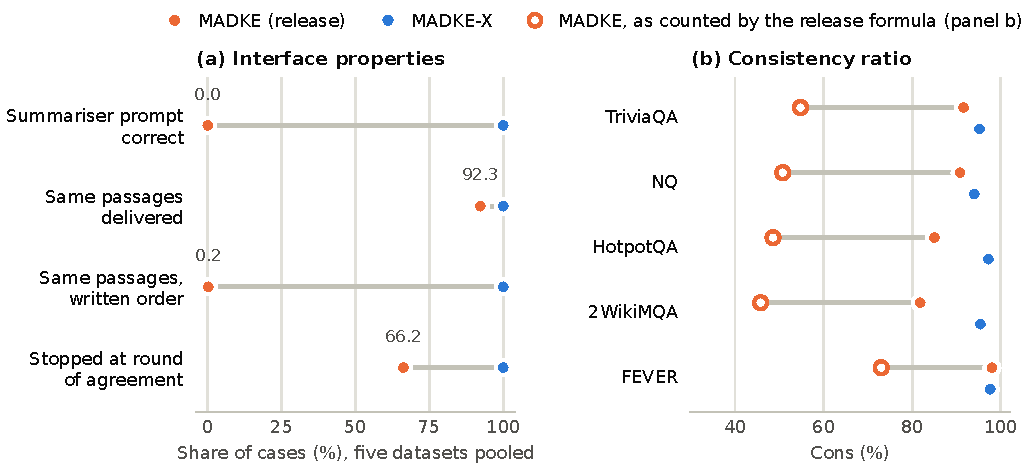
\includegraphics[width=\textwidth]{fig_interface}
\caption{Interface behaviour under scripted agents. (a) Share of cases in which each property holds, pooled over the five datasets; the numbers are the values of MADKE. (b) Consistency ratio of the same debates: as stated in the judge replies, as counted by the evaluation formula of the release, and as computed by MADKE-X.}
\label{fig:interface}
\end{figure}

\subsection{Debate statistics (RQ1)}
Table~\ref{tab:consistency} and Figure~\ref{fig:interface}b separate two losses in the consistency ratio of the release. The reference value is the share of debates in which a judge reply states agreement. Over the five datasets it is \VConsTrueRel\% in the re-run of the release. The verdicts that the release recognised give \VConsPipeRel\%: the difference is the agreement that the literal test missed (finding C4). The evaluation formula of the release then reports \VConsFormRel\%, because it cannot count an agreement of the last round (finding C5). On the single datasets the formula reports \VConsGapMin{} to \VConsGapMax{} points less than the judge replies state.

For MADKE-X the first two columns agree on every dataset, as invariant D2 requires, and the formula of the release would lose only \VConsGapXMin{} to \VConsGapXMax{} points, since few debates of MADKE-X reach the last round at all. Co2 shows the same pattern at a lower level. The level itself carries no meaning here, because the answers come from scripts. Nor do the differences between the two systems in the first column: the two systems hold different debates over different pools.

% generated by paper_assets.py -- do not edit by hand
\begin{table}[!htbp]
\centering
\small
\caption{Debate statistics under scripted agents (500 questions per dataset). \emph{Judge replies}: agreement as stated in the judge replies, read with the verdict parser of Eq.~\eqref{eq:verdict}; this is the reference value. \emph{Stored verdicts}: Eq.~\eqref{eq:cons} applied to the verdicts that steered the debate. \emph{Release formula}: the computation of the released evaluation script. Correctness in Co2 is exact match; the scripted answers are not model answers, so the level of Co2 carries no meaning and only the differences between the three columns are of interest.}
\label{tab:consistency}
\setlength{\tabcolsep}{4pt}
\begin{tabular}{llrrrrrr}
\toprule
 & & \multicolumn{3}{c}{Cons (\%)} & \multicolumn{3}{c}{Co2 (\%)} \\
\cmidrule(lr){3-5}\cmidrule(lr){6-8}
Dataset & System & \shortstack{judge\\replies} & \shortstack{stored\\verdicts} & \shortstack{release\\formula} & \shortstack{judge\\replies} & \shortstack{stored\\verdicts} & \shortstack{release\\formula} \\
\midrule
\multirow{2}{*}{TriviaQA} & MADKE & 91.6 & 76.2 & 54.8 & 14.6 & 12.0 & 10.0 \\
 & MADKE-X & 95.2 & 95.2 & 93.6 & 16.2 & 16.2 & 15.8 \\
\midrule
\multirow{2}{*}{NQ} & MADKE & 90.8 & 73.6 & 50.8 & 7.2 & 6.0 & 4.0 \\
 & MADKE-X & 94.0 & 94.0 & 91.8 & 8.0 & 8.0 & 7.8 \\
\midrule
\multirow{2}{*}{HotpotQA} & MADKE & 85.0 & 67.0 & 48.6 & 3.6 & 3.0 & 2.4 \\
 & MADKE-X & 97.2 & 97.2 & 96.2 & 3.8 & 3.8 & 3.8 \\
\midrule
\multirow{2}{*}{2WikiMQA} & MADKE & 81.8 & 68.4 & 45.8 & 0.0 & 0.0 & 0.0 \\
 & MADKE-X & 95.4 & 95.4 & 93.6 & 0.0 & 0.0 & 0.0 \\
\midrule
\multirow{2}{*}{FEVER} & MADKE & 98.0 & 81.4 & 73.0 & 33.2 & 28.6 & 25.2 \\
 & MADKE-X & 97.6 & 97.6 & 96.6 & 33.4 & 33.4 & 33.2 \\
\bottomrule
\end{tabular}
\end{table}


\subsection{Failure handling (RQ1)}
\label{sec:r_failure}
Table~\ref{tab:failure} reports the fault-injection experiment on the first \VFailN{} questions of every dataset, in which each scripted call fails with a probability of \VFailRate\%. The release marks no question as failed. It scores \VFailScoredRel{} of the \VFailNAll{} questions although at least one of their calls failed, \VFailScoredRelMin{} to \VFailScoredRelMax{} per dataset; in these debates an error message took the place of a selection, an answer, a verdict or the summary. MADKE-X stops a question at its first failed call and marks it as failed. This happened for \VFailFlaggedX{} questions, \VFailFlaggedXMin{} to \VFailFlaggedXMax{} per dataset, and the scores were computed from the questions that remained. The release meets more failures than MADKE-X because it makes more calls per question and keeps calling after a failure. With a failure rate of zero both systems complete every question.

% generated by paper_assets.py -- do not edit by hand
\begin{table}[!htbp]
\centering
\small
\caption{Fault injection: every scripted call fails with probability 2\%. MADKE passes the error text on as a reply and scores the question; MADKE-X marks the question as failed and excludes it from the scores.}
\label{tab:failure}
\setlength{\tabcolsep}{6pt}
\resizebox{\textwidth}{!}{%
\begin{tabular}{lrrrrrr}
\toprule
 & & \multicolumn{2}{c}{MADKE} & \multicolumn{3}{c}{MADKE-X} \\
\cmidrule(lr){3-4}\cmidrule(lr){5-7}
Dataset & Questions & \shortstack{marked\\failed} & \shortstack{scored although\\a call failed} & \shortstack{marked\\failed} & \shortstack{completed\\and scored} & \shortstack{scored although\\a call failed} \\
\midrule
TriviaQA & 100 & 0 & 18 & 15 & 85 & 0 \\
NQ & 100 & 0 & 19 & 16 & 84 & 0 \\
HotpotQA & 100 & 0 & 19 & 16 & 84 & 0 \\
2WikiMQA & 100 & 0 & 24 & 12 & 88 & 0 \\
FEVER & 100 & 0 & 20 & 9 & 91 & 0 \\
\midrule
All five & 500 & 0 & 100 & 68 & 432 & 0 \\
\bottomrule
\end{tabular}%
}
\end{table}


\subsection{Evidence ordering (RQ2)}
\label{sec:r_order}
Table~\ref{tab:ordering} and Figure~\ref{fig:ordering} report how early an answer-bearing passage appears under each ordering, and Table~\ref{tab:paired} gives the paired test of the RRF order against the order of the release. FEVER and the questions with a yes or no answer are not included, for the reason given in Section~\ref{sec:design}.

The release lists all Wikipedia passages before any Google passage, whatever the question. On TriviaQA, HotpotQA and 2WikiMultihopQA this order is worse than a random order of the pool at $k=3$: an answer-bearing passage is among the first three for \VCovThreeOrigTQA\%, \VCovThreeOrigHQA\% and \VCovThreeOrigWMQ\% of the questions, against random expectations of \VCovThreeRandTQA\%, \VCovThreeRandHQA\% and \VCovThreeRandWMQ\%. The cause is the position of the Google snippets. They are short, they often contain the answer string, and they come last. The interleaved order does nothing but alternate the two sources, and it already lifts cov@3 to \VCovThreeInterTQA\%, \VCovThreeInterHQA\% and \VCovThreeInterWMQ\% on these datasets. NQ is the exception: its Wikipedia order beats the random expectation (\VCovThreeOrigNQ\% against \VCovThreeRandNQ\%), so the dense retriever serves this dataset well.

% generated by paper_assets.py -- do not edit by hand
\begin{table}[!htbp]
\centering
\small
\caption{Position of the first answer-bearing passage under five orderings (cov@$k$ in percent of the questions with a span answer; best value per dataset in bold). \emph{Release order}: ten Wikipedia passages followed by five Google passages. The other orderings rearrange the MADKE-X pool; \emph{Random} is the exact expectation over all orders of that pool.}
\label{tab:ordering}
\begin{tabular}{llrrrr}
\toprule
Dataset & Ordering & cov@1 & cov@3 & cov@5 & MRR \\
\midrule
\multirow{5}{*}{\shortstack[l]{TriviaQA\\($n=500$)}} & Release order & 39.2 & 52.0 & 57.0 & 0.486 \\
 & Interleaved & 39.2 & 72.6 & 78.8 & 0.574 \\
 & BM25 only & 54.8 & 75.8 & \textbf{80.2} & 0.657 \\
 & RRF (MADKE-X) & \textbf{56.4} & \textbf{76.0} & 79.2 & \textbf{0.666} \\
 & Random (expected) & 39.3 & 66.5 & 76.1 & 0.545 \\
\midrule
\multirow{5}{*}{\shortstack[l]{NQ\\($n=500$)}} & Release order & \textbf{47.2} & 60.4 & 67.6 & 0.565 \\
 & Interleaved & \textbf{47.2} & \textbf{69.4} & \textbf{76.2} & \textbf{0.600} \\
 & BM25 only & 35.4 & 63.2 & 73.8 & 0.512 \\
 & RRF (MADKE-X) & 45.0 & 66.4 & 75.4 & 0.578 \\
 & Random (expected) & 30.1 & 57.3 & 69.7 & 0.467 \\
\midrule
\multirow{5}{*}{\shortstack[l]{HotpotQA\\($n=465$)}} & Release order & 16.1 & 21.7 & 24.9 & 0.219 \\
 & Interleaved & 16.1 & 34.6 & 40.2 & 0.275 \\
 & BM25 only & 22.6 & 39.4 & 45.2 & 0.318 \\
 & RRF (MADKE-X) & \textbf{27.5} & \textbf{41.5} & \textbf{45.8} & \textbf{0.348} \\
 & Random (expected) & 13.4 & 28.7 & 37.2 & 0.234 \\
\midrule
\multirow{5}{*}{\shortstack[l]{2WikiMQA\\($n=468$)}} & Release order & 6.4 & 11.8 & 15.2 & 0.119 \\
 & Interleaved & 6.4 & 22.0 & 29.1 & 0.167 \\
 & BM25 only & \textbf{18.8} & \textbf{26.5} & 32.1 & \textbf{0.242} \\
 & RRF (MADKE-X) & 16.2 & 26.3 & \textbf{32.3} & 0.228 \\
 & Random (expected) & 7.2 & 17.9 & 25.8 & 0.152 \\
\bottomrule
\end{tabular}
\end{table}


\begin{figure}[!htbp]
\centering
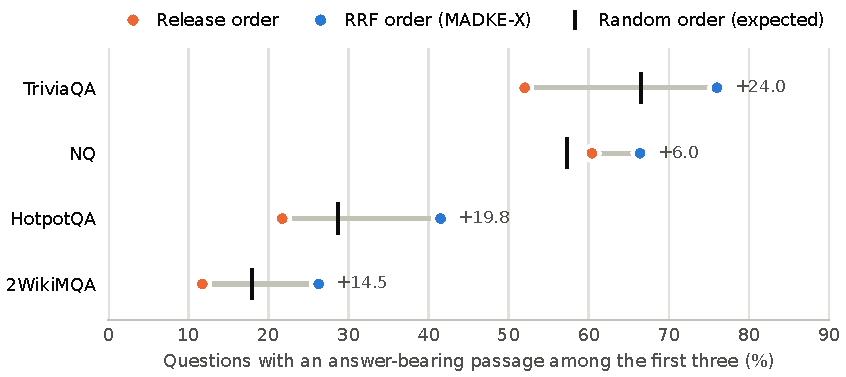
\includegraphics[width=0.88\textwidth]{fig_ordering}
\caption{Questions with an answer-bearing passage among the first three passages of the listing, under the order of the release and under the RRF order of MADKE-X. The vertical mark is the expectation under a random order of the MADKE-X pool; the number is the gain in percentage points.}
\label{fig:ordering}
\end{figure}

BM25 alone and RRF are both better than the order of the release at $k=3$ on all four datasets, and RRF is above the random expectation on all four. RRF reaches a cov@3 of \VCovThreeRrfTQA\%, \VCovThreeRrfNQ\%, \VCovThreeRrfHQA\% and \VCovThreeRrfWMQ\%, which are gains of \VGainTQA, \VGainNQ, \VGainHQA{} and \VGainWMQ{} points. All four gains are significant under the exact McNemar test, also after Holm correction (largest adjusted $p=\VHolmMax$; Table~\ref{tab:paired}). The mean reciprocal rank moves the same way, for instance from \VMrrOrigTQA{} to \VMrrRrfTQA{} on TriviaQA and from \VMrrOrigHQA{} to \VMrrRrfHQA{} on HotpotQA.

% generated by paper_assets.py -- do not edit by hand
\begin{table}[!htbp]
\centering
\small
\caption{Paired comparison of the RRF order with the release order on cov@3. \emph{RRF only} and \emph{Release only} count the questions that have an answer-bearing passage among the first three under one ordering but not the other.}
\label{tab:paired}
\setlength{\tabcolsep}{5pt}
\resizebox{\textwidth}{!}{%
\begin{tabular}{lrrrrccc}
\toprule
Dataset & $n$ & \shortstack{RRF\\only} & \shortstack{Release\\only} & \shortstack{Gain\\(points)} & \shortstack{95\% bootstrap\\interval} & \shortstack{Exact\\McNemar $p$} & \shortstack{Holm-adjusted\\$p$} \\
\midrule
TriviaQA & 500 & 130 & 10 & $+24.0$ & [19.8, 28.4] & $8.9\times10^{-28}$ & $3.6\times10^{-27}$ \\
NQ & 500 & 75 & 45 & $+6.0$ & [1.6, 10.4] & $0.008$ & $0.008$ \\
HotpotQA & 465 & 100 & 8 & $+19.8$ & [16.1, 23.9] & $2.4\times10^{-21}$ & $7.1\times10^{-21}$ \\
2WikiMQA & 468 & 84 & 16 & $+14.5$ & [10.5, 18.6] & $2.6\times10^{-12}$ & $5.2\times10^{-12}$ \\
\bottomrule
\end{tabular}%
}
\end{table}


RRF is not the best ordering in every cell of Table~\ref{tab:ordering}. On NQ the interleaved order is ahead at $k=3$ and $k=5$, and BM25 alone is slightly ahead in a few cells on TriviaQA and 2WikiMultihopQA. What distinguishes RRF is that it is never far behind. Over the twelve coverage cells of the table it trails the best ordering by at most \VWorstGapRrf{} points, whereas BM25 alone trails by up to \VWorstGapBm{} points, the interleaved order by up to \VWorstGapInter{} and the order of the release by up to \VWorstGapOrig. The weak cell of BM25 is the first position on NQ. The Wikipedia order has an answer-bearing passage there for \VCovOneOrigNQ\% of the questions, BM25 alone for \VCovOneBmNQ\% and RRF for \VCovOneRrfNQ\%. Fusing the source rank with the lexical rank guards against the questions whose terms are a poor guide and keeps the gains where the original order is uninformative.

\subsection{Pool size, coverage and cost (RQ2, RQ3)}
\label{sec:r_cost}
The gains in ordering are not free in coverage. Table~\ref{tab:pool} and Figure~\ref{fig:cost}b show that the step from the default pool of the release to the specified pool lowers the share of questions with any answer-bearing passage by \VCoverLossTQA{} points on TriviaQA, \VCoverLossNQ{} on NQ, \VCoverLossHQA{} on HotpotQA and \VCoverLossWMQ{} on 2WikiMultihopQA. The questions that are lost have their only answer-bearing passage among the Wikipedia passages ranked sixth to tenth. De-duplication removes \VDupMin{} to \VDupMax{} passages per dataset, \VDupTotal{} in all, and does not change coverage.

% generated by paper_assets.py -- do not edit by hand
\begin{table}[!htbp]
\centering
\small
\caption{Evidence pool of the release (ten Wikipedia and five Google passages) and of MADKE-X (five and five, de-duplicated) on the shipped files; means over 500 questions. Listing tokens: size of the evidence listing of one selection call (cl100k\_base tokenizer). Coverage: share of the questions with a span answer whose pool holds an answer-bearing passage; it is not defined for the verdict labels of FEVER.}
\label{tab:pool}
\setlength{\tabcolsep}{5pt}
\resizebox{\textwidth}{!}{%
\begin{tabular}{lrrrrrrrr}
\toprule
 & \multicolumn{2}{c}{Passages} & \multicolumn{3}{c}{Listing tokens} & \multicolumn{2}{c}{Coverage (\%)} & Duplicates \\
\cmidrule(lr){2-3}\cmidrule(lr){4-6}\cmidrule(lr){7-8}
Dataset & MADKE & MADKE-X & MADKE & MADKE-X & $-$\% & MADKE & MADKE-X & removed \\
\midrule
TriviaQA & 14.54 & 9.52 & 1,671 & 923 & 44.8 & 83.8 & 83.0 & 12 \\
NQ & 14.99 & 9.97 & 1,669 & 930 & 44.3 & 86.6 & 83.6 & 12 \\
HotpotQA & 14.93 & 9.90 & 1,713 & 951 & 44.5 & 51.6 & 48.2 & 13 \\
2WikiMQA & 14.79 & 9.76 & 1,761 & 977 & 44.5 & 41.2 & 38.0 & 16 \\
FEVER & 14.98 & 9.97 & 1,685 & 935 & 44.5 & n/a & n/a & 7 \\
\bottomrule
\end{tabular}%
}
\end{table}


On the cost side (Table~\ref{tab:pool}, Figure~\ref{fig:cost}a), the specified pool shortens the evidence listing of a selection call from about 1,700 tokens to between \VTokXTQA{} and \VTokXWMQ{} tokens, a reduction of \VTokRedMin{} to \VTokRedMax\%. Nearly all of it comes from the size of the pool; de-duplication alone shortens the listing by at most \VTokRedSpecMax\%. The saving is relative to the default of the release. A user who already runs MADKE with five Wikipedia passages gains almost nothing in tokens from MADKE-X.

Building a pool takes \VBuildXMin{} to \VBuildXMax\,ms per question, against about a microsecond for slicing two lists, and the reference statistics of a file are built in \VIndexMsMin{} to \VIndexMsMax\,ms. The pools of the 500 questions of a dataset occupy \VMemXMin{} to \VMemXMax\,MB with their manifests; the sliced lists of the release only reference the loaded data and occupy \VMemRelMax\,MB. Next to a model call that takes seconds, these costs do not matter.

\begin{figure}[!htbp]
\centering
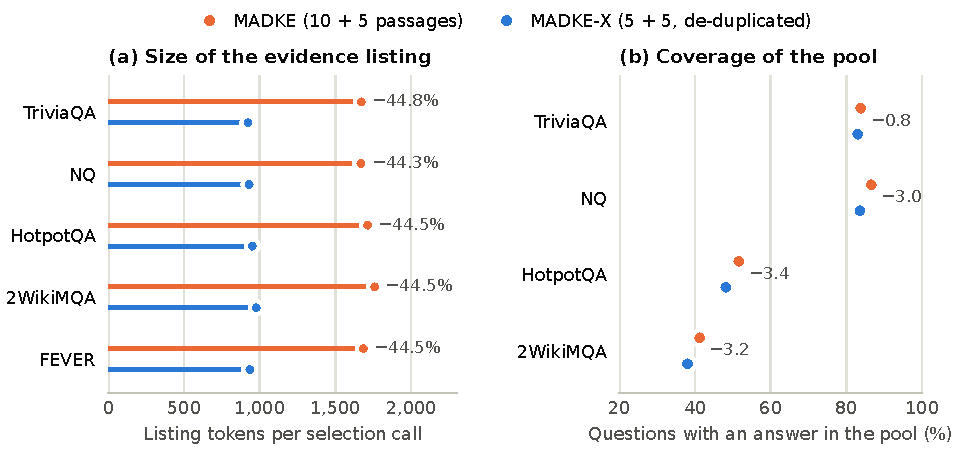
\includegraphics[width=\textwidth]{fig_cost}
\caption{The benefit and the price of the specified pool. (a) Tokens of the evidence listing of one selection call, with the reduction in percent. (b) Share of questions for which the pool contains an answer-bearing passage, with the loss in percentage points.}
\label{fig:cost}
\end{figure}

The debates of the two systems also differ in length. Under scripted agents the release needed \VRoundsRel{} rounds and \VCallsRel{} model calls per question on average, MADKE-X \VRoundsX{} rounds and \VCallsX{} calls, and the input of a question, counted over the system and user messages of all its calls, fell from \VInTokRel{} to \VInTokX{} tokens (\VInTokRed\% less). Two causes act together, the shorter listing and the earlier stop. Their shares depend on how the scripted judge words its verdicts, so the corresponding figure for a language model has to come from the live runs.

\subsection{Trace, citations and verification (RQ3)}
Over the \VNQuestions{} scripted debates of MADKE-X, the identifiers stored in the trace satisfied the bounds and the cap in every selection (invariant I3), all \VCiteParsed{} citations pointed to a passage of the pool that an agent had selected, and the stored support status was reproduced from the trace for every record (invariant I5). For FEVER, and for the \VVerdictAnswers{} questions of the other datasets that were answered with ``yes'' or ``no'', the status is \emph{not applicable}. When the scripted summariser cites the passages that contain its answer, at least \VSupXMin\% of the applicable answers are supported at the end on each dataset. The verification step was triggered \VVerCalls{} times in these runs; \VVerAdopt{} second answers were adopted, and the scripted verifier abstained \VVerAbst{} times.

A summariser that cites well leaves the verification step little to do, so a stress test was run with a careless one (Table~\ref{tab:stress}, Figure~\ref{fig:verification}). This scripted summariser always cites the first listed passage. Its first answer is supported for only \VStressBeforeMin{} to \VStressBeforeMax\% of the questions, and the verification step is called \VStressCalls{} times. In \VStressSame{} of these calls the second reply keeps the answer and cites a passage that contains it. In \VStressNew{} calls it gives a different answer that a listed passage supports, and in \VStressAbst{} it abstains, in which case the first answer stays. No second reply was itself unsupported, and no answer that was supported at first was touched. The support rate ends at \VStressAfterMin\% or higher on every dataset. These counts come from scripts. They show that the step behaves as Eq.~\eqref{eq:verify} specifies and say nothing about how often a real model will be helped.

% generated by paper_assets.py -- do not edit by hand
\begin{table}[!htbp]
\centering
\small
\caption{Stress test of the bounded verification step: a scripted summariser that always cites the first listed passage, whether or not it contains the answer (500 questions per dataset). Applicable: completed questions whose final answer is not a verdict.}
\label{tab:stress}
\setlength{\tabcolsep}{5pt}
\resizebox{\textwidth}{!}{%
\begin{tabular}{lrrrrrrrr}
\toprule
 & & & & \multicolumn{3}{c}{Outcome of the call} & & \\
\cmidrule(lr){5-7}
Dataset & \shortstack{Appli-\\cable} & \shortstack{Supported\\at first (\%)} & \shortstack{Verification\\calls} & \shortstack{adopted,\\same answer} & \shortstack{adopted,\\new answer} & abstained & \shortstack{Supported at\\the end (\%)} & \shortstack{Supported\\answers changed} \\
\midrule
TriviaQA & 499 & 70.3 & 148 & 144 & 2 & 2 & 99.6 & 0 \\
NQ & 500 & 61.8 & 191 & 188 & 1 & 2 & 99.6 & 0 \\
HotpotQA & 500 & 74.4 & 128 & 126 & 0 & 2 & 99.6 & 0 \\
2WikiMQA & 499 & 65.1 & 174 & 170 & 2 & 2 & 99.6 & 0 \\
\bottomrule
\end{tabular}%
}
\end{table}


\begin{figure}[!htbp]
\centering
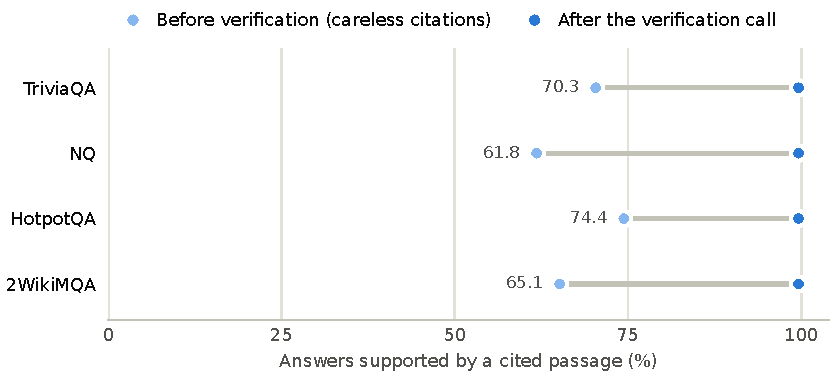
\includegraphics[width=0.88\textwidth]{fig_verification}
\caption{Stress test of the bounded verification step with a scripted summariser that always cites the first listed passage: share of answers supported by a cited passage before and after the step. The numbers are the values before the step.}
\label{fig:verification}
\end{figure}

\subsection{Summary of the offline results}
RQ1 is answered positively. Under identical scripted agents MADKE-X meets every invariant, gives the summariser a correct prompt, delivers the selected passages in every case and ends every debate in the round of agreement, and its debate statistics equal the direct count. The release fails each of these properties for a measurable share of the cases, and it scores questions whose calls failed. RQ2 is answered positively with a qualification. The RRF order lists answer-bearing passages earlier on all four question-answering datasets, with paired significance, and the smaller pool that the MADKE paper specifies costs up to \VCoverLossMax{} points of coverage. RQ3 is answered positively: the evidence listing shrinks by \VTokRedMean\% relative to the default of the release, the added time and memory are negligible, and the trace reproduces what the pipeline did. None of these results says anything about accuracy, which is the subject of the next section.

\section{End-to-end comparison with a live model}
\label{sec:live}

This section addresses RQ4. Accuracy can be measured only with a language model, and a fair comparison requires that MADKE and MADKE-X answer the same questions with the same model, the same debate prompts and the same sampling parameters. The release is therefore run again under the harness of MADKE-X. The published numbers are not used as the baseline, because they come from other models and another infrastructure.

\subsection{Choice of comparison}
The original evaluation used three backbones. Two of them are reached through paid commercial interfaces, and the third, with 72 billion parameters, cannot be served on freely available hardware. The comparison here is restricted to systems whose code is public and can be run under identical conditions: MADKE, through the logic of its release, and MADKE-X. The single-agent and debate baselines of the original paper (SP, CoT, SC, RAG and MAD) are not part of the release. Implementing them anew would add differences in prompts and parsing that could not be told apart from the methods themselves. Their published numbers are reported for reference in Table~\ref{tab:published} and are kept out of the comparison of the two re-run systems.

\subsection{Models and infrastructure}
Two open-weight models serve as backbones. Qwen1.5-32B-Chat \cite{bai2023qwen} is one of the backbones of the MADKE paper. Qwen2.5-7B-Instruct \cite{yang2024qwen25} is smaller and more recent, and with it all questions can be processed in the compute that is available. Both models are served by Ollama with 4-bit quantised weights through its OpenAI-compatible endpoint, on a cloud notebook with two NVIDIA T4 GPUs of 16\,GB each. For the smaller model one server runs on each GPU and the datasets are split between the two.

The temperature is 0.5 as in MADKE, and a reply is limited to 512 tokens. The context window is set to 8,192 tokens. The longest prompt of either system is the selection prompt of the release, which stays below 2,800 tokens of the cl100k\_base tokenizer. Every call passes through the client of Eq.~\eqref{eq:call}. A run starts only after a test request to the endpoint has succeeded, and it stops by itself when five consecutive questions contain failed calls, so that an unreachable server cannot produce an empty table of results. Questions are processed in batches by index. Each finished question is written to a checkpoint at once, and an interrupted run resumes without repeating questions. The reference statistics of the governor do not depend on the batch, so a run in batches builds the same pools as a single run.

The serving set-up was tried with two questions per dataset for both models and both systems, using an earlier version of the code. All calls succeeded. A trial of this size permits no statement on accuracy, and its outcomes are not reported.

\subsection{Results}
Table~\ref{tab:live} reports EM and F1 for the four question-answering datasets, EM for FEVER, and Cons and Co2, for both systems on the same questions. The number of completed and of failed questions is stated in the table. Paired exact McNemar tests on EM and 95\% bootstrap intervals are reported with the final numbers. Cells marked ``--'' are pending: the corresponding runs had not finished when this version of the manuscript was prepared. No value in the table is estimated or extrapolated.

% generated by paper_assets.py -- do not edit by hand
\begin{table}[!htbp]
\centering
\small
\caption{Live comparison of MADKE (release re-run) and MADKE-X on identical questions, with Qwen2.5-7B-Instruct and Qwen1.5-32B-Chat as backbones. $n$: completed questions per dataset; failed: questions excluded because a model call failed; EM and F1 in percent over the completed questions; Cons and Co2 by Eq.~\eqref{eq:cons}, averaged over the five datasets. ``--'': the run had not finished when this version of the manuscript was prepared; no value is estimated.}
\label{tab:live}
\setlength{\tabcolsep}{3pt}
\resizebox{\textwidth}{!}{%
\begin{tabular}{llrrccccccccccc}
\toprule
 & & & & \multicolumn{2}{c}{TriviaQA} & \multicolumn{2}{c}{NQ} & \multicolumn{2}{c}{HotpotQA} & \multicolumn{2}{c}{2WikiMQA} & FEVER & & \\
\cmidrule(lr){5-6}\cmidrule(lr){7-8}\cmidrule(lr){9-10}\cmidrule(lr){11-12}\cmidrule(lr){13-13}
Backbone & System & $n$ & failed & EM & F1 & EM & F1 & EM & F1 & EM & F1 & EM & Cons & Co2 \\
\midrule
\multirow{2}{*}{Qwen2.5-7B} & MADKE & -- & -- & -- & -- & -- & -- & -- & -- & -- & -- & -- & -- & -- \\
 & MADKE-X & -- & -- & -- & -- & -- & -- & -- & -- & -- & -- & -- & -- & -- \\
\midrule
\multirow{2}{*}{Qwen1.5-32B} & MADKE & -- & -- & -- & -- & -- & -- & -- & -- & -- & -- & -- & -- & -- \\
 & MADKE-X & -- & -- & -- & -- & -- & -- & -- & -- & -- & -- & -- & -- & -- \\
\bottomrule
\end{tabular}%
}
\end{table}


\subsection{Published results for reference}
Table~\ref{tab:published} copies the main results of the MADKE paper \cite{wang2025madke} from Table~2 of its arXiv version (arXiv:2312.04854v2). The values were not measured again. They document the size of the differences that the original evaluation reports and are not a comparison with Table~\ref{tab:live}: they were obtained with other backbones, the G4 columns rest on a GPT-4 judge, and the code that produced them cannot be identified with the public release (Section~\ref{sec:audit}).

% generated by paper_assets.py -- do not edit by hand
\begin{table}[!htbp]
\centering
\footnotesize
\caption{Results published for MADKE and its baselines \cite{wang2025madke}, copied from Table~2 of the arXiv version (v2) without re-measurement. F1 and GPT-4 score (G4) for the four question-answering datasets, exact match for FEVER. SP: standard prompting; CoT: chain of thought; SC: self-consistency; RAG: retrieval-augmented generation; MAD: multi-agent debate.}
\label{tab:published}
\setlength{\tabcolsep}{4pt}
\resizebox{\textwidth}{!}{%
\begin{tabular}{llccccccccc}
\toprule
 & & \multicolumn{2}{c}{TriviaQA} & \multicolumn{2}{c}{NQ} & \multicolumn{2}{c}{HotpotQA} & \multicolumn{2}{c}{2WikiMQA} & FEVER \\
\cmidrule(lr){3-4}\cmidrule(lr){5-6}\cmidrule(lr){7-8}\cmidrule(lr){9-10}\cmidrule(lr){11-11}
Backbone & Method & F1 & G4 & F1 & G4 & F1 & G4 & F1 & G4 & EM \\
\midrule
\multirow{6}{*}{GPT-3.5-Turbo} & SP & 0.761 & 0.778 & 0.390 & 0.532 & 0.331 & 0.384 & 0.190 & 0.210 & 0.548 \\
 & CoT & 0.715 & 0.772 & 0.418 & 0.588 & 0.333 & 0.410 & 0.165 & 0.190 & 0.556 \\
 & SC & 0.756 & 0.818 & 0.431 & 0.622 & 0.342 & 0.408 & 0.175 & 0.206 & 0.560 \\
 & RAG & 0.768 & 0.824 & 0.450 & 0.436 & 0.423 & 0.498 & 0.204 & 0.228 & 0.646 \\
 & MAD & 0.712 & 0.798 & 0.401 & 0.648 & 0.287 & 0.394 & 0.133 & 0.186 & 0.548 \\
 & MADKE & 0.728 & 0.830 & 0.453 & 0.736 & 0.405 & 0.542 & 0.205 & 0.274 & 0.612 \\
\midrule
\multirow{6}{*}{Qwen1.5-32B-Chat} & SP & 0.581 & 0.632 & 0.295 & 0.462 & 0.311 & 0.384 & 0.207 & 0.220 & 0.536 \\
 & CoT & 0.587 & 0.644 & 0.276 & 0.452 & 0.315 & 0.382 & 0.220 & 0.228 & 0.546 \\
 & SC & 0.583 & 0.628 & 0.276 & 0.442 & 0.312 & 0.386 & 0.203 & 0.222 & 0.540 \\
 & RAG & 0.446 & 0.554 & 0.269 & 0.436 & 0.309 & 0.420 & 0.183 & 0.248 & 0.664 \\
 & MAD & 0.630 & 0.704 & 0.321 & 0.566 & 0.363 & 0.482 & 0.256 & 0.286 & 0.520 \\
 & MADKE & 0.763 & 0.838 & 0.475 & 0.724 & 0.450 & 0.570 & 0.258 & 0.314 & 0.646 \\
\midrule
\multirow{6}{*}{Qwen1.5-72B-Chat} & SP & 0.665 & 0.706 & 0.378 & 0.550 & 0.332 & 0.428 & 0.226 & 0.260 & 0.596 \\
 & CoT & 0.715 & 0.776 & 0.406 & 0.648 & 0.431 & 0.514 & 0.275 & 0.324 & 0.625 \\
 & SC & 0.659 & 0.700 & 0.369 & 0.548 & 0.336 & 0.430 & 0.207 & 0.242 & 0.596 \\
 & RAG & 0.662 & 0.762 & 0.333 & 0.710 & 0.438 & 0.538 & 0.217 & 0.304 & 0.668 \\
 & MAD & 0.703 & 0.796 & 0.376 & 0.660 & 0.397 & 0.548 & 0.274 & 0.344 & 0.516 \\
 & MADKE & 0.787 & 0.874 & 0.479 & 0.748 & 0.495 & 0.622 & 0.284 & 0.350 & 0.686 \\
\midrule
\multirow{1}{*}{GPT-4-Turbo} & SP & 0.828 & 0.902 & 0.459 & 0.692 & 0.472 & 0.566 & 0.265 & 0.284 & 0.608 \\
\bottomrule
\end{tabular}%
}
\end{table}


Several published margins are small for the number of questions. Figure~\ref{fig:power} takes each of the \VPowN{} margins between MADKE and its strongest baseline on the share metrics of Table~\ref{tab:published} (GPT-4 score and FEVER exact match) and gives the number of questions per method that Eq.~\eqref{eq:power} requires for 80\% power at the 5\% level. \VPowOver{} of the \VPowN{} margins need more than 500 questions and \VPowOverTwoK{} need more than 2,000; in \VPowBelow{} cases MADKE lies below its strongest baseline. The published evaluation scored all methods on one sample of questions per dataset, so a paired test on its per-question outcomes would be more sensitive than this calculation, but those outcomes are not published. The calculation explains why the live comparison of this study is paired and why its primary test pools the five datasets.

\begin{figure}[!htbp]
\centering
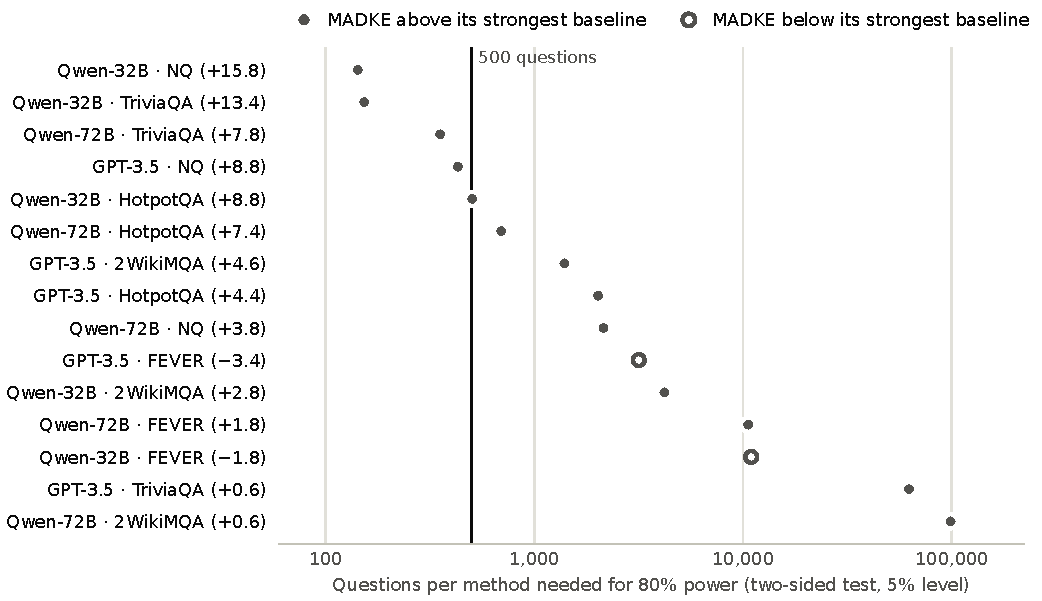
\includegraphics[width=0.92\textwidth]{fig_power}
\caption{Questions per method needed to detect each published margin between MADKE and its strongest baseline with 80\% power (two-sided test of two proportions at the 5\% level, Eq.~\ref{eq:power}). The label gives the backbone, the dataset and the margin in percentage points. The vertical line marks the 500 questions of the benchmark files.}
\label{fig:power}
\end{figure}

\subsection{Analyses that the live records support}
The records of a live run contain everything that the offline analyses use, so the following quantities can be computed from them without further model calls: the share of selection replies that the parser of the release would have read differently, and the share of agreeing judge replies that its verdict test would have missed, both for a real model; the share of questions on which the agents agreed on a wrong answer ($\mathrm{Cons}-\mathrm{Co2}$); the distribution of the support status for correct and for incorrect answers; the number of questions on which verification was triggered and adopted; and the number of rounds, calls and input tokens per question for both systems. An ablation that switches the components of MADKE-X on one at a time needs further runs and is planned for the smaller model, which processes a dataset fastest.

\section{Discussion}
\label{sec:discussion}

\paragraph{What the results establish}
The offline results establish two things of different kinds. The first concerns the data. On the shipped files, the order in which the release lists the evidence places answer-bearing passages among the first three less often than chance would on three of four datasets, and a reordering that needs no labels repairs this. No agent takes part in this measurement, so it holds for any backbone. The second concerns the code. Under replies of known content, the release departs from the specification of the paper in a share of the cases, and MADKE-X does not. How large that share is with a real model depends on how the model formats its replies, and this study does not know it. A model that always writes \texttt{[Yes]} and never writes a list in one bracket would trigger neither finding C3 nor C4. The swapped summariser prompt, the consistency formula and the handling of errors are different: they do not depend on the format of any reply.

\paragraph{Why the order matters for a debate}
In MADKE an agent chooses at most three passages from a listing that opens with five to ten Wikipedia passages, while the short Google snippets that most often contain the answer string come last. Language models use long contexts unevenly \cite{liu2024lost}, so an agent is more likely to pick early passages that help less, and the debate then rests on weaker evidence. The RRF order puts an answer-bearing passage among the first three for \VGainMin{} to \VGainMax{} percentage points more questions, from the question and the retrieval rank alone. Whether agents turn the better listing into better answers is what the live comparison measures; the offline result shows that the opportunity exists. The comparison of orderings also carries a caution. Simply interleaving the two sources achieves most of the gain, and on NQ it achieves more than RRF at three passages. The merit of the fusion is that it holds up on every dataset. It is not the best choice on each.

\paragraph{The price of the specified pool}
The pool that the MADKE paper specifies makes the listing \VTokRedMean\% shorter than the default of the release, and it removes the only answer-bearing passage for \VCoverLossMin{} to \VCoverLossMax\% of the questions. A faithful implementation has to follow the specification, and the pool size remains configurable through $w$ and $g$ in Eq.~\eqref{eq:pool}. On HotpotQA and 2WikiMultihopQA about half of the questions or fewer have an answer-bearing passage in either pool. Retrieval, and not debate, limits these datasets, and iterative retrieval \cite{trivedi2023ircot} is the natural next step for them.

\paragraph{Traceability as a property of the system}
For a question-answering system in use, showing why an answer was given matters apart from accuracy. The trace of MADKE-X records what the pipeline did and is in that sense faithful to the process \cite{jacovi2020faithful}: every answer can be inspected, failures are counted, and a comparison can be recomputed from the stored records. The lexical support check is the weakest part, and deliberately so. It detects that the answer string is missing from the cited passages. It does not establish that a passage entails the answer, and it rejects correct paraphrases. A learned attribution model \cite{rashkin2023attribution,gao2023alce} could replace it without touching the rest of the pipeline. The verification step built on the check inherits its limits. It can never replace a supported answer and costs at most one call. Whether supported answers are more often correct than unsupported ones can be read directly from the live records, which store the status next to the gold answers.

\paragraph{What is not shown}
This study does not show that MADKE-X answers more questions correctly than MADKE. That claim rests on the live runs of Table~\ref{tab:live}. Nor does it show that the published results of MADKE are wrong. The findings concern the public code, and the published shares fit an evaluation of all 500 questions.

\section{Threats to validity}
\label{sec:threats}

\paragraph{Internal validity}
The offline comparison drives both systems with scripted replies, so differences between them are caused by the code. The scripts, however, write a chosen set of formats, and a real model may write formats that neither parser anticipates. The parsers of MADKE-X record every identifier and every verdict they cannot use, so such cases stay visible in the trace. Reading the selection from the end of the reply is a convention and can fail: a reply that states its selection first and afterwards discusses further passages in brackets is read wrongly by both parsers once it names more than three passages. The number of replies with dropped identifiers is therefore reported for every live run. The MADKE baseline is the logic of the release reproduced inside the harness of MADKE-X and not the original scripts. The reproduction follows the released code statement by statement for each finding of Table~\ref{tab:defects}, but differences in infrastructure, such as the model server, cannot be excluded. Finally, the summariser prompt of MADKE-X differs from that of MADKE in more than the request for citations: for the question-answering datasets it gives one worked example where MADKE gives three. A difference in accuracy between the two full systems can thus be assigned to a single component only through the ablation.

\paragraph{Construct validity}
Coverage and the support check rest on a normalised match of whole words with a gold answer. A passage that states the answer in other words is counted as not answer-bearing, and a passage that contains the answer string by coincidence is counted as answer-bearing. Tokens are counted with the cl100k\_base tokenizer and not with the tokenizer of the Qwen models; the relative reductions should carry over, the absolute numbers will differ. EM and F1 are standard for extractive question answering \cite{rajpurkar2016squad}, but they penalise a correct answer that is phrased differently from every gold alias. The GPT-4 score of the original evaluation was not reproduced, and Co2 with exact match is stricter than the published Co2.

\paragraph{External validity}
The live comparison uses open-weight Qwen models with 4-bit quantisation and not the commercial models of the original evaluation, and quantisation can change the behaviour of a model. Other model families, larger pools, other retrieval sources and other numbers of agents or rounds may give different results. The medical dataset of the original evaluation is not shipped and is not covered. The BM25 statistics come from the passages of the benchmark file; in a deployed system they would come from the retrieval corpus.

\paragraph{Conclusion validity}
Several published margins are smaller than 500 questions can resolve (Figure~\ref{fig:power}). Differences on single datasets in the live comparison are therefore treated as exploratory, the paired test pooled over the datasets with Holm correction is the primary test, and every reported difference comes with its confidence interval. The offline rates of the interface properties depend on the format shares of the scripts and must not be read as estimates for a language model. The published baseline values of Table~\ref{tab:published} serve as reference only and are evidence neither for nor against one of the two systems.

\section{Conclusion}
\label{sec:conclusion}

This study introduced MADKE-X, a governed debate framework that turns knowledge-enhanced multi-agent debate from an exchange of prompts that nobody can inspect into a process that is specified, checked and recorded at every step. A failure-aware interface layer, an evidence governor, a decision trace with citations and a bounded verification step were each defined by an equation, and the effect of each equation was measured on the unaltered benchmark files that are shipped with MADKE, the debate system on which the framework was built and against which it was tested.

On these files, the evidence governor places an answer-bearing passage among the first three passages of the listing for \VGainMin{} to \VGainMax{} percentage points more questions on the four question-answering datasets, with paired significance on each. It shortens the evidence listing of every selection call by \VTokRedMean\% relative to the default of the release, at a cost of less than a millisecond per question and of up to \VCoverLossMax{} points of coverage. Under identical scripted agents, MADKE-X passes all \VInvChecksAll{} pipeline checks. The summariser prompt holds the question in every case, where the release has it in none. Every selection reaches the agent that made it, where the release loses the \VSetBadRel{} selections that are written as a list. Every debate ends in the round of agreement, against \VStopPctRel\% for the release, and the consistency ratio equals the direct count, where the formula of the release reports \VConsGapMin{} to \VConsGapMax{} points too little. Each answer of MADKE-X carries a trace of the evidence delivered, the verdicts, the cited passages and a support status, and the verification step raises the number of supported answers without changing a supported one.

None of the four components depends on the debate design, the prompts or the backbone model, so the framework can in principle be placed around other debate systems that draw on retrieved evidence. The end-to-end accuracy of both systems is compared on the same questions with open-weight Qwen models under a paired protocol, and Table~\ref{tab:live} holds the results as the runs finish. Three extensions follow from the limitations of this study: a learned attribution model in place of the lexical support check, iterative retrieval for the multi-hop questions whose pools contain no answer-bearing passage, and a comparison with further model families on more questions.

\section*{CRediT authorship contribution statement}
\textbf{Muhammad Ali:} Conceptualization, Methodology, Software, Investigation, Writing -- original draft. \textbf{Muhammad Talha:} Validation, Investigation, Data curation, Writing -- review \& editing. \textcolor{red}{[To the authors: confirm these roles before submission and delete this note.]}

\section*{Declaration of competing interest}
The authors declare that they have no known competing financial interests or personal relationships that could have appeared to influence the work reported in this paper.

\section*{Declaration of generative AI and AI-assisted technologies in the writing process}
During the preparation of this work the authors used Claude (Anthropic) in order to assist with programming, with the analysis scripts and with the drafting and language editing of the manuscript. After using this tool, the authors reviewed and edited the content as needed and take full responsibility for the content of the published article.

\section*{Data and code availability}
The code of MADKE-X, the scripts that generate every table, figure and number of this manuscript, the per-question records of the offline experiments and the SHA-256 checksums of the data are released with the manuscript. The datasets are those distributed with the MADKE repository \cite{madke2025code} and are used unmodified.


\bibliographystyle{elsarticle-num}
\bibliography{references}

\end{document}
